%%%%%%%%%%%%%%%%%%%%%%%%%%%%%%%%%%%%%%%%%%%%%%%%%%%%%%%%%%
%
% Vzor pro sazbu kvalifikační práce
%
% Západočeská univerzita v Plzni
% Fakulta aplikovaných věd
% Katedra informatiky a výpočetní techniky
%
% Petr Lobaz, lobaz@kiv.zcu.cz, 2016/03/14
%
%%%%%%%%%%%%%%%%%%%%%%%%%%%%%%%%%%%%%%%%%%%%%%%%%%%%%%%%%%

% Možné jazyky práce: czech, english
% Možné typy práce: BP (bakalářská), DP (diplomová)
\documentclass[czech,BP]{thesiskiv}

% Definujte údaje pro vstupní strany
%
% Jméno a příjmení; kvůli textu prohlášení určete, 
% zda jde o mužské, nebo ženské jméno.
\author{Vojtěch Danišík}
\declarationmale

%alternativa: 
%\declarationfemale

% Název práce
\title{Generátor a parser formulářů recenzí příspěvků na konferenci TSD}

% 
% Texty abstraktů (anglicky, česky)
% 

%The text of the abstract (in English). It contains the English translation of the thesis title and a short description of the thesis.
\abstracttexten{Generator and Parser of Submission Review Forms for the TSD Conference.
\newline The goal of this thesis is to create easily integrable PHP module into already existing informational system for TSD conference management. Task of the module is to create evaluative form in the PDF format and process it after loading it back into the system. First part of thesis deeply explains standard format PDF and forms created with PDF. Existing libraries for processing and generating the scientific contribution are explained afterward. Second part of thesis focuses on implementation of mentioned libraries into the web portal of TSD conference. Module has been tested by users of conference system. There has been used multiple PDF explorers during testing. Results of the tests are part of the thesis.}


%Text abstraktu (česky). Obsahuje krátkou anotaci (cca 10 řádek) v češtině. Budete ji potřebovat i při vyplňování údajů o bakalářské práci ve STAGu. Český i anglický abstrakt by měly být na stejné stránce a měly by si obsahem co možná nejvíce odpovídat (samozřejmě není možný doslovný překlad!).
\abstracttextcz{Cílem bakalářské práce je vytvořit jednoduše integrovatelný PHP modul do již existujícího informačního systému pro správu konference TSD. Úkolem modulu bude vytvořit hodnotící fomulář ve formátu PDF a následně ho po nahrání do systému zpracovat. První část práce důkladně vysvětluje standardní formát PDF a formuláře vytvořené v~PDF. Následně jsou popsány existující PHP knihovny pro generování a zpracování PDF formuláře daného vědeckého příspěvku. Druhá část práce se věnuje implementaci vybraných knihoven do webového portálu konference TSD. Modul byl otestován uživateli konferenčního systému. Při testování bylo použito více PDF prohlížečů. Výsledky testování jsou součástí této práce.}

% Na titulní stranu a do textu prohlášení se automaticky vkládá 
% aktuální rok, resp. datum. Můžete je změnit:
%\titlepageyear{2016}
%\declarationdate{1. března 2016}

% Ve zvláštních případech je možné ovlivnit i ostatní texty:
%
%\university{Západočeská univerzita v Plzni}
%\faculty{Fakulta aplikovaných věd}
%\department{Katedra informatiky a výpočetní techniky}
%\subject{Bakalářská práce}
%\titlepagetown{Plzeň}
%\declarationtown{Plzni}

%%%%%%%%%%%%%%%%%%%%%%%%%%%%%%%%%%%%%%%%%%%%%%%%%%%%%%%%%%
%
% DODATEČNÉ BALÍČKY PRO SAZBU
% Jejich užívání či neužívání záleží na libovůli autora 
% práce
%
%%%%%%%%%%%%%%%%%%%%%%%%%%%%%%%%%%%%%%%%%%%%%%%%%%%%%%%%%%

% Zařadit literaturu do obsahu
\usepackage[nottoc,notlot,notlof]{tocbibind}

% Umožňuje vkládání obrázků
\usepackage[pdftex]{graphicx}

% Odkazy v PDF jsou aktivní; navíc se automaticky vkládá
% balíček 'url', který umožňuje např. dělení slov
% uvnitř URL
\usepackage[pdftex]{hyperref}
\hypersetup{colorlinks=true,
  unicode=true,
  linkcolor=black,
  citecolor=black,
  urlcolor=black,
  bookmarksopen=true}

% Při používání citačního stylu csplainnatkiv
% (odvozen z csplainnat, http://repo.or.cz/w/csplainnat.git)
% lze snadno modifikovat vzhled citací v textu
\usepackage[numbers,sort&compress]{natbib}

\usepackage{svg}
\usepackage{textcomp}
\usepackage{amsmath}
\usepackage{listings,xcolor}
\usepackage{mathtools}
\usepackage[final]{pdfpages}
\usepackage{verbatim}

\definecolor{dkgreen}{rgb}{0,.6,0}
%\definecolor{dkblue}{rgb}{0,0,.6}
%\definecolor{dkyellow}{cmyk}{0,0,.8,.3}

\lstdefinestyle{phpstyle}{
language = php,
frame = single,
basicstyle = \footnotesize\ttfamily,
breaklines = true,
showtabs = false,
showstringspaces = false,
stringstyle = \color{red},
identifierstyle = \color{blue},
commentstyle = \color{gray},
emph =[1]{function},
emphstyle =[1]\color{dkgreen}\bfseries,
emph =[2]{generate_offline_review_form, process_offline_review_form, upload_to_DB_offline_review_form, (, )},
emphstyle =[2]\color{black}
}

%%%%%%%%%%%%%%%%%%%%%%%%%%%%%%%%%%%%%%%%%%%%%%%%%%%%%%%%%%
%
% VLASTNÍ TEXT PRÁCE
%
%%%%%%%%%%%%%%%%%%%%%%%%%%%%%%%%%%%%%%%%%%%%%%%%%%%%%%%%%%
\begin{document}
%
\maketitle
\tableofcontents

\thispagestyle{empty}
\setcounter{page}{0} 
%CHAPTER
\chapter{Úvod}
TSD (\textbf{T}ext, \textbf{S}peech and \textbf{D}ialogue) je mezinárodní konference zabývající se například problémy zpracování, překladu a rozpoznávání přirozeného jazyka nebo analýzou řeči. Mezi nejčastěji probíraná témata se řadí například rozpoznávání řeči, modelování řeči,textové korpusy, značkování textu a mnoho dalších. Konference se koná každý rok v~září a místo konání se střídá mezi Brnem (pořadatelem je Fakulta informatiky Masarykovy Univerzity) a Plzní (pořadatelem je Fakulta aplikovaných věd Západočeské univerzity v~Plzni). Tento rok bude konference organizována právě Západočeskou univerzitou, a poprvé se bude konat za hranicemi České Republiky, přesněji ve Slovinsku ve městě Ljubljana.
\par
Ke konferenci existuje webový portál, na nějž jsou od uživatelů nahrávány vědecké příspěvky. Tyto příspěvky jsou poté hodnoceny recenzenty (převážně členy programového výboru) formou online formuláře a na základě konečného hodnocení jednotlivých parametrů a na doporučení recenzentů jsou tyto příspěvky schváleny organizátorem a mohou být prezentovány na konferenci. Modul, vytvářený autorem, bude implementován do webového portálu konference TSD.
\par
Cílem této práce je prostudovat strukturu PDF formátu, který je pro vytváření editovatelných formulářů nejvhodnější a byl vybrán zadávajícím jako standard, tak i funkcionalitu volně dostupných PHP knihoven pro generování a parsování PDF souborů obsahujících editovatelný formulář, aby existovala možnost ohodnocení daného vědeckého příspěvku i v~místech, kde není dostupné internetové připojení, neboli off-line. Vytvořený PDF soubor musí obsahovat hodnotící formulář se všemi hodnotícími parametry doplněný o~text vědeckého příspěvku. Pro generování a parsování musí být použity výhradně knihovny v~jazyce PHP, jelikož není vhodné využívat aplikace třetích stran spustitelné z~terminálu. Modul musí být nezávislý na platformě a lze ho upravovat v~jakémkoliv PDF prohlížeči. Před vytvořením modulu na testovací verzi webového portálu bude potřeba projít zdrojové soubory webového portálu pro seznámení s~již existujícími funkcionalitami a zařadit do portálu i náš modul. Z~dřívějších let je zde naimplementován totožný modul pro generování a parsování PDF souborů, bohužel tento modul nesplňuje veškeré body zadání právě z~důvodu použití nevhodného parseru.
 
%CHAPTER
\chapter{Formát PDF}
Formát \textbf{PDF} (\textbf{P}ortable \textbf{D}ocument \textbf{F}ormat) je souborový formát vyvinutý společností Adobe v roce 1992. PDF formát byl vyvinut za účelem konzistentní prezentace dokumentů (spustitelné na více zařízeních a různých platformách). Díky konzistenci lze dosáhnout toho, že PDF soubor vytvořený a uložený v systému Windows bude zobrazen totožně na systémech Mac, na všech distribucích Linuxu nezávisle na použitém PDF prohlížeči (Adobe Reader, Foxit a další).
\par 
V PDF souboru lze uchovávat velice širokou škálu dat, včetně formátovaného textu, vektorové grafiky a rastrových obrazů, nebo například informace o rozložení, velikosti a tvaru stránky. Informace definující umístění jednotlivých položek (jsou zde zahrnuty i editovací objekty pro formuláře) na stránce jsou zde uloženy též. Do dokumentu lze ukládat i metadata. Metadata jsou informace uložené v hlavičce souboru a lze do nich uložit název dokumentu, autora dokumentu, předmět a klíčová slova. Je zde možnost uložit heslo, aby byl dokument přístupný pouze autorizovaným uživatelům. Všechny tyto informace jsou uloženy ve standardním formátu \cite{PDFTechTerms, PDFWhatIs}.

%SECTION
\section{Objekty}
PDF Objekty jsou základním stavebním kamenem pro uchovávání dat v dokumentu. Množinou PDF objektů lze reprezentovat bitmapové a vektorové objekty, barevné prostory, text, fonty aj. \cite{PDFExplained}.
%SUBSECTION
\subsection{Základní objekty}
V PDF můžeme najít celkem 5 základních objektů:
	\begin{itemize}
		\item \textbf{Celá a reálná čísla} - Celá čísla jsou reprezentována jako jedno nebo více desetinných čísel z rozsahu 0..9 se znaménkem + nebo - před číslem. Reálné číslo je celé číslo rozšířené o desetinnou část s ideálně jedním desetinným číslem (reálná čísla nelze popsat exponenciálním způsobem). Přesnost a rozsah celých a reálných čísel je definován jednotlivými implementacemi PDF. V některých implementacích platí pravidlo které přetypuje celé číslo na reálné po přesáhnutí předem daného rozsahu.
		\item \textbf{Řetězce} - Řetězec je reprezentován jako množina po sobě jdoucích bytů vepsaných mezi jednoduché závorky. Jako příklad lze uvést: \textit{(Hello, World!)}. Pro zobrazení zpětného lomítka a jednoduchých závorek je potřeba před tyto znaky přidat zpětné lomítko pro jejich správné zobrazení v dokumentu. V tabulce \ref{fig:table_escaped} lze vidět využití zpětného lomítka pro zobrazení odřádkovacích znaků:
			\begin{table}[h!]
			\centering
			\begin{tabular}{|l|l|} 
			\hline
			\textbf{Sekvence znaků}    & \textbf{Význam}                \\ 
			\hline
			\textit{\textbackslash{}n} & \textit{Line feed (LF)}        \\ 
			\hline
			\textit{\textbackslash{}r} & \textit{Carriage return (CR)}  \\ 
			\hline
			\textit{\textbackslash{}t} & \textit{Tab}                   \\ 
			\hline
			\textit{\textbackslash{}b} & Backspace                      \\
			\hline
			\end{tabular}
			\caption{Odřádkovací sekvence znaků}
			\label{fig:table_escaped}
			\end{table}
		\newline Řetězce můžou být reprezentovány i jako sekvence hexadecimálních čísel vložených mezi znaky \textbf{<} a \textbf{>}. 
		\newline Jako příklad lze uvést: \textit{<4F6EFF00> \textrightarrow 0x4F, 0x6E, 0xFF, 0x00}.

		\item \textbf{Jména} - Jméno je reprezentováno jako sloučení zpětného lomítka a řetězce (př. \textit{/Jmeno}). Za jméno se pokládá i zpětné lomítko bez řetězce. Pokud bychom potřebovali nadefinovat v dokumentu jméno, jenž bude obsahovat mezery, musíme do řetězce přidat i sekvenci znaků \textbf{\#20}, jelikož v ASCII tabulce je hexadecimální hodnota 20 vyjádřena jako prázdný znak. Jména jsou case-sensitive, proto \textit{/Jmeno} a \textit{/jmeno} jsou rozdílná jména. Jeho využití v PDF je prosté, slouží jako klíče ve slovnících a pro definice složitějších (vícehodnotových) objektů.
		\item \textbf{Boolean (pravdivostní) hodnoty} - Logické hodnoty \textbf{true}/\textbf{false} a vyskytuje se v jednotlivých záznamech ve slovníku jako příznak.
		\item \textbf{Hodnota null} - Nabývá hodnot \textit{f} (free) nebo \textit{n} (use) a vyjadřuje, zda je objekt vyobrazen v dokumentu.
	\end{itemize}
%SUBSECTION
\subsection{Složené objekty}	
Složený objekt je takový objekt, který obsahuje seřazenou/neseřazenou množinu základních objektů i množinu složených objektů.
	\begin{itemize}
		\item \textbf{Pole} - Pole je v PDF reprezentováno jako seřazená množina základních i složených PDF objektů (v poli může být uložen například i slovník nebo pole) nezávisle na typech (v poli lze uchovávat například řetězec a číslo zároveň). Hodnoty pole jsou vloženy mezi znaky \textbf{[} a \textbf{]}.
		\item \textbf{Slovníky} - Slovník se skládá z množiny dvou hodnot: klíče a hodnoty, pomocí kterých se slovník namapuje. Klíč je reprezentován pomocí \textbf{jména}, zatímco hodnota může být kterýkoliv PDF objekt, povoleny jsou i slovníky nebo pole. Slovníky jsou uloženy mezi znaky \textbf{<<} a \textbf{>>}.
		\item \textbf{Datové proudy} - Datové proudy slouží především pro uložení binárních dat a skoro ve všech případech jsou zkomprimovány různými kombinacemi algoritmů, které jsou popsány v kapitole \ref{komprese}, proto datové proudy musí být zároveň i nepřímým odkazem. Skládají se ze slovníků a části binárních dat. Slovník je využit pro ukládání parametrů binárních dat, jako například délka binárních dat aj.
	\end{itemize}
%SUBSECTION
\subsection{Linkovací objekty}
PDF objekty můžou být různě velké. Pokud je objekt až příliš veliký, pak jsou v kódu dokumentu využity nepřímé odkazy. Na obrázku \ref{fig:indirect_reference} si lze všimnout využití nepřímých odkazů ve slovníku. 
	\begin{figure}[h!]
	\centering
	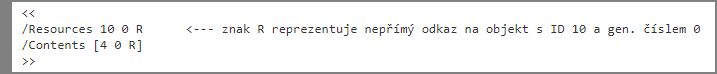
\includegraphics[width=15cm]{img/pdf_indirect_reference}
	\caption{Ukázka nepřímého odkazu}
	\label{fig:indirect_reference}
	\end{figure}

%SECTION
\section{Komprese dat v PDF}
\label{komprese}
PDF soubory moho být poměrně kompaktní, o mnoho menší než ekvivalentní postscriptové soubory. Tato vlastnost je dosažena nejen lepší strukturou dat, ale i díky kompresním algoritmům, které jsou velice efektivní. Typ komprese dat PDF souboru lze zjistit pomocí textového editoru, který dokáže zpracovat binární data, vyhledáním klíčového slova \textbf{/Filter}. Níže jsou popsány kompresní algoritmy využívané v PDF \cite{PDFPrepressure}.
\begin{itemize}
	\item \textbf{CCITT G3/G4} - Algoritmus je bezeztrátový a využívá se pro vykreslení černobílých obrázků.
	\item \textbf{JPEG} - JPEG algoritmus může být jak ztrátový, tak i bezeztrátový. V Acrobatu se využívá pouze ztrátový s 5 stupni komprese. Využívá se pro barevné a šedotónové obrázky.
	\item \textbf{JPEG2000} - Rychlejší algoritmus na bázi JPEGu. Víceméně se nepoužívá, jelikož není kompatibilní se staršímy systémy a vysokýmy nároky na procesor.
	\item \textbf{Flate} - Bezeztrátový algoritmus, vychází z kompresních algoritmů LZ77 a Huffmanova kódování.
	\item \textbf{JBIG2} - Alternativní k CCITT. V Dnešní době se nevyužívá z důvodu pomalejší komprese než je u jeho protějšku.
	\item \textbf{LZW} - Komprimací LZW algoritmem lze dosáhnout až o polovinu menší velikosti díky komprimaci veškerého textu a operátorů v souboru.
	\item \textbf{RLE} - Bezeztrátový algoritmus pro vykreslování černobílých obrázků. Nahrazen efektivnějším algoritmem CCITT.
	\item \textbf{ZIP} - Bezeztrátový algoritmus, učinější než jeho protějšek LZW.
\end{itemize}

%SECTION
\section{Vnitřní struktura PDF}
Vnitřní reprezentace PDF souboru je rozdělena na sekce, které jsou znázorněny na obrázku \ref{fig:pdf_internal_structure}.

\begin{figure}[h!]
\centering
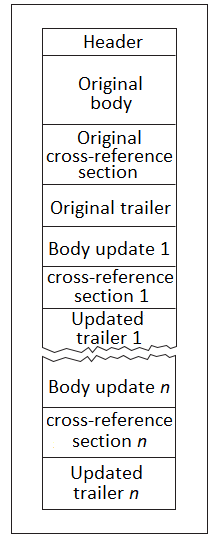
\includegraphics[width=4cm]{img/pdf_internal_structure}
\caption{Interní struktura PDF souboru}
\label{fig:pdf_internal_structure}
\end{figure}

Z obrázku lze vyčíst, že se zde vyskytují 4 hlavní sekce: \textit{Header, Body, Cross-reference a trailer}. Díky jedné z vlastností PDF formátu se při úpravě souboru staré sekce neodstraní, místo toho se pouze na jeho konci vytvoří nové sekce \cite{PDFInfoSec}.
\begin{itemize}
	\item \textbf{Header} - Hlavička souboru je uložena na první řádce, obsahující primárně použitou verzi PDF.
	\begin{figure}[h!]
	\centering
	
\includegraphics[width=15cm]{img/pdf_hlavicka}
	\caption{Ukázka hlavičky}
	\label{fig:pdf_header}
	\end{figure}
	
	\item \textbf{Body} - V těle dokumentu jsou uložena veškerá data objektů reprezentující celý dokument. Objekty jsou referencovány v tabulce Cross-reference z důvodu rozprostření částí dat patřících k danému objektu po celé sekci.Pokud se v dokumentu vyskytuje jeden obrázek/zvukový záznam vícekrát než jednou, tak se poté všechny objekty reprezentující obrázky odkazují na jednu množinu dat \cite{PDFAdobe}.
	\begin{figure}[h!]
	\centering
	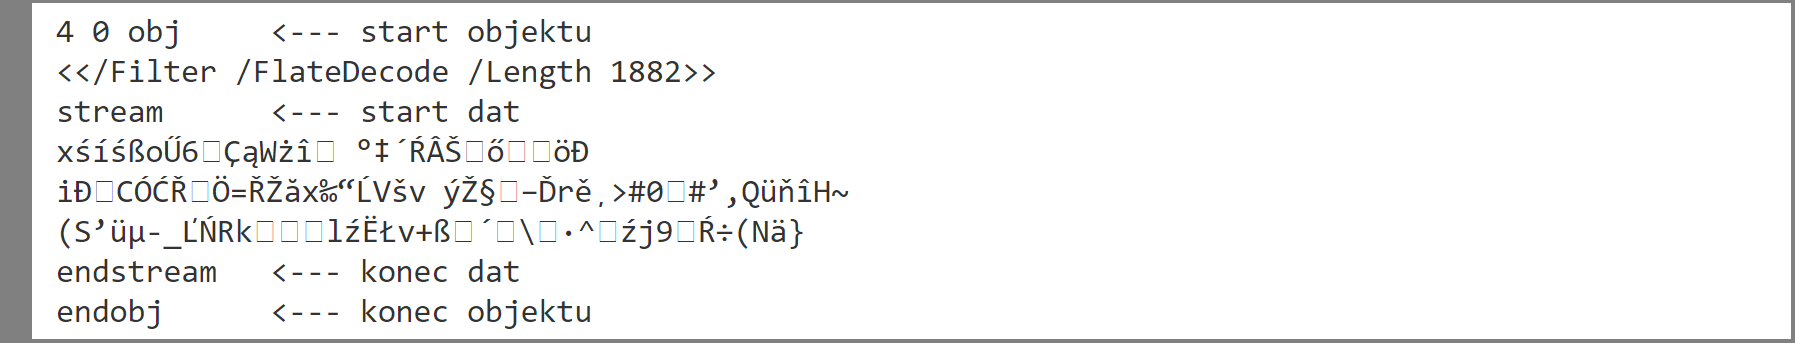
\includegraphics[width=15cm]{img/pdf_body}
	\caption{Ukázka dat objektu}
	\label{fig:pdf_body}
	\end{figure}

	\item \textbf{Cross-reference table} - Jinak nazývána \textbf{xref} je tabulka obsahující reference na veškeré objekty uložené v těle a v kódu začíná řetězcem \textit{xref}. Reference uložená v tabulce je reprezentována na 2 řádcích pomocí řetězce a skládá se z 5 částí o celkové velikosti 20 bytů včetně oddělovačů \textit{CRLF}:
	\begin{itemize}
		\item \textit{Číslo objektu} - Jednoznačný číselný identifikátor objektu.
		\item \textit{Počet subobjektů} - Počet částí daného objektu vyskytujícího se v dokumentu.
		\item \textit{Začátek objektu} - Tvoří většinu řetězce (prvních 10 bytů) a určuje offset od začátku PDF dokumentu až po začátek daného objektu.
		\item \textit{Generační číslo objektu} - Vyjadřuje jak často byl objekt vymazán při úpravě dokumentu. 
		\item \textit{Identifikátor využití} - Nabývá hodnot \textit{f} (free) nebo \textit{n} (use) a vyjadřuje, zda je objekt vyobrazen v dokumentu.
	\end{itemize}
	\begin{figure}[h!]
	\centering
	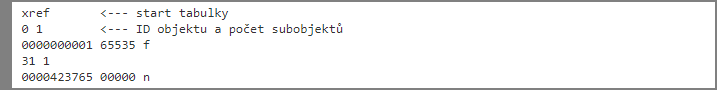
\includegraphics[width=15cm]{img/pdf_xref}
	\caption{Ukázka jednoduché xref tabulky}
	\label{fig:pdf_xref}
	\end{figure}

	\item \textbf{Trailer} -  Trailer je seznam informací, ze kterých lze snadno zjistit například velikost nebo umístění xref tabulky. Trailer může obsahovat tyto elementy:
	\begin{itemize}
		\item \textit{Size} - Udává počet objektů referencovaných v xref tabulce. 
		\item \textit{Prev} - Offset od začátku dokumentu k předchozí xref tabulce.
		\item \textit{Root} - Odkazuje na objekt obsahující informace ohledně katalogu xref tabulek.
		\item \textit{Encrypt} - Specifikuje komprimující algoritmus použití pro daný dokument.
		\item \textit{Info} - Obsahuje dodatečné informace ohledně katalogu xref tabulek.
		\item \textit{ID} - 2-bytový identifikátor PDF dokumentu.
		\item \textit{XrefStm} - Offset od začátku dokumentu až k dekódovanému xref streamu. Využívá se pouze u hybridně-referencovaných souborů pouze tehdy, kdy hledaný objekt není nalezen v xref tabulce (před tím, než se volá element \textit{Prev}). 
	\end{itemize}
	\begin{figure}[h!]
	\centering
	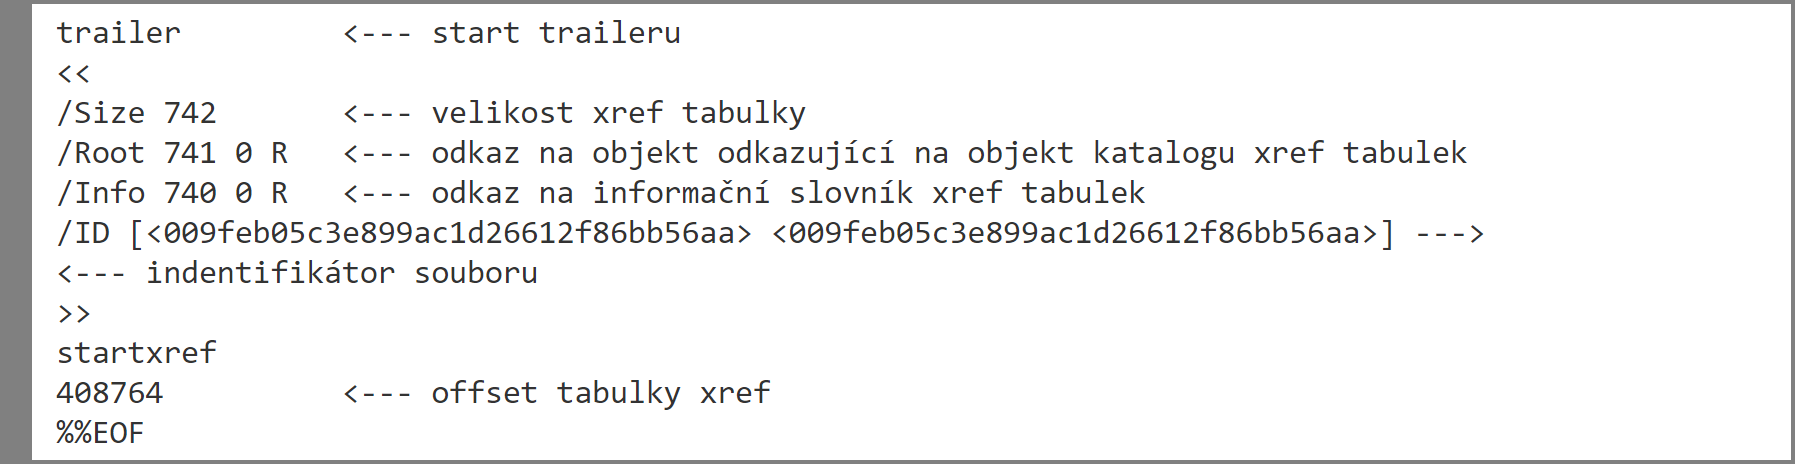
\includegraphics[width=15cm]{img/pdf_trailer}
	\caption{Ukázka traileru}
	\label{fig:pdf_trailer}
	\end{figure}
\end{itemize}
%SECTION
\section{PDF formuláře}
Pod pojmem formulář si lze představit dokumenty, které od svých uživatelů vyžadují vyplnění určitých údajů. Mezi nejznámější dokumenty lze například uvést daňová přiznání, oznamovací tiskopisy, dotazníky, složenky aj. Ruční vyplňování i jejich následné zpracování bývá obvykle pracné a zdlouhavé, proto je v dnešní době výhodnější využívat interaktivní elektronické formuláře. Základní výhoda těchto formulářů spočívá ve snažším vyplňování, zpracování lze jednoduše zautomatizovat a také se díky elektronické podobě zvedne úspora papíru a financí vynaložených na tisk formulářů.  Mezi nejčastější formuláře, které lze potkat na internetu, jsou ve formátu HTML a lidé se s nima setkávají každodenně (ať už to jsou jednoduché přihlašovací formuláře stránek nebo různé dotazníky na určitá témata). Nevýhoda těchto formulářů je v jejich závislosti na internetovém připojení. 
\par
Proto firma Adobe přišla se svým řešením, interaktivním PDF formulářem, který lze vyplňovat kdekoliv nezávisle na internetovém připojení. Mezi další výhody PDF formulářů patří elektronický podpis (lze s ním potvrzovat smlouvy z domova), zabezpečení (dokument se otevře až po zadání správného hesla, neautorizovaným uživatelům je přístup zamítnut) aj. Tyto formuláře obsahují stejné interaktivní prvky jako mají HTML formuláře viz kapitola \ref{zakladni_prvky}. Pro generování PDF formulářů lze využít kterýkoliv programovací jazyk, který podporuje práci s PDF soubory (například \textit{PHP}, \textit{Java}), produkty firmy Adobe (například \textit{Adobe Acrobat}) nebo lze použít i nekomerční aplikace typu \textit{TeX} nebo \textit{pdfmarks}.
\par
Tvorba formulářů je jedna věc, druhá věc je jejich zpracování (získání dat vyplněných od uživatele). Mezi nejznámější nástroje pro zpracování vyplněných dat patří určitě nástroj \textit{FDF Toolkit} od firmy Adobe. Tento nástroj je zcela zdarma a umožňuje vytvářet orientovaná řešení pro zpracování dat v jazycích \textit{C/C++}, \textit{ActiveX}, \textit{Java} a \textit{Perl}. Jsou-li data odeslána v HTML, lze k jejich zpracování využít nástroje určené pro formáty \textit{CGI}, \textit{PHP} aj. \cite{PDFForm}.
%SUBSECTION
\subsection{Základní prvky} \label{zakladni_prvky}
Jednotlivé formulářové prvky mohou mít přiřazeny nejrůznější atributy a jsou reprezentovány jako PDF objekty. Tyto atributy lze rozdělit do následujících skupin: \textbf{Vzhled} (definovaný vzhled prvku), \textbf{Akce} (po kliknutí na prvek se provede daná akce), \textbf{Formát} (typ fontu textu aj.), \textbf{Ověřování dat} (akceptovatelný formát vstupu) a \textbf{Výpočty} (matematické operace použité při práci se vstupy z jiných prvků) \cite{PDFFormElements}. 
\par
Ve formuláři se může vyskytovat až 7 různých prvků viz obrázek \ref{fig:form_elements}:
	\begin{figure}[h!]
	\centering
	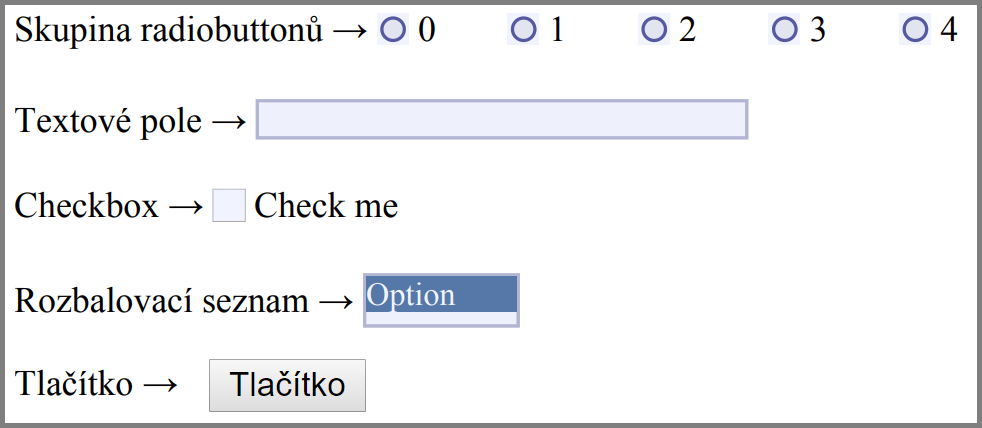
\includegraphics[width=9cm]{img/pdf_form_elements}
	\caption{Základní prvky vyskytující se v PDF}
	\label{fig:form_elements}
	\end{figure}
	\begin{itemize}
	\item \textbf{Textové pole} - Slouží k vyplnění textu. Jako příklad lze uvést například klasický přihlašovací formulář, který obsahuje 2 textové pole, jedno pro zadání uživatelského jména a druhé (upravené, místo textu se zobrazují pouze speciální znaky pro zakrytí zadaného textu)  pro zadání hesla. Při vytváření lze předvyplnit toto pole výchozím textem, lze omezit maximální počet znaků vkládaných do pole a jejich formát. Pole může být uzamčeno a může sloužit i jako informační položka.
	\item \textbf{Tlačítko} - Účel tohoto prvku je spouštění zvolených akcí, které se po kliknutí na tlačítko mají provést, tudíž se označují jako hlavní řídící prvek každého formuláře. Tlačítko se skládá převážně z ikonky a textu, případně mu může být nastaven externí obrázek.
	\item \textbf{Seznam} - Zobrazuje seznam položek v rolovacím okně, ze kterého lze současně označit jeden nebo více položek (s využitím klávesy \textit{Shift} nebo \textit{Ctrl}). Pro seznamy lze nastavit filtry, které budou seznam třídit podle předem daných parametrů a zobrazí položky na základě těchto filtrů.
	\item \textbf{Kombinované pole} - Kombinované pole je ve své podstatě seznam prvků, ale liší se ve výběru položek. V kombinovaném poli lze vybrat pouze jeden aktivní prvek, ostatní budou zakázány. Platí zde pravidla s tříděním pprvků odle filtrů.
	\item \textbf{Přepínací tlačítka} - Jinak označované jako \textbf{radio-buttony} je seznam tlačítek, ve kterém uživatel vybírá pouze jednu z nabízených hodnot.
	\item \textbf{Zaškrtávací pole} - Jedná se o indikační prvek umožňující současný výběr více položek. V odborném prostředí se označuje jako \textbf{Checkbox}.
	\item \textbf{Podpis} - Pomocí tohoto prvku lze do dokumentu vložit elektronický podpis.
	\end{itemize}
%CHAPTER
\chapter{Knihovny}
V~programování můžeme knihovnu definovat jako kolekci předem zkompilovaných procedur, funkcí (v~objektovém programování i třídy a objekty), konstant a datových typů. Knihovna by měla být následně i dobře zdokumentována pro její snadnější zakomponování do již existujících modulů (při používání nezdokumentovaných knihoven se musí provádět takzvaný reverse engineering pro zjištění všech procedur a funkcí, nebo vyhledávat už hotová řešení na internetu). 
\par
Knihovny jsou z~technického hlediska rozděleny do 2 skupin, které se následně rozdělují do 2 podskupin:
	\begin{itemize}
	\item \textbf{Rozdělení z~hlediska způsobu propojení s~programem:}
		\begin{itemize}
		\item \textit{Statická knihovna} -- Zdrojový kód knihovny je v~průběhu překládání zkopírován do výsledného programu pomocí kompilátoru. Největší výhoda statických knihoven spočívá v~jistotě, že všechny potřebné knihovny budou přítomny ve výsledném programu, proto nikdy nemůže nastat situace nazvaná \textit{dependency hell (DLL Hell)}, která značí nepřítomnost jedné nebo více knihoven, které jsou využívány jinou knihovnou, nebo také může značit nadbytečné závislosti knihoven, které nejsou ve výsledku využity.
		\item \textit{Dynamická knihovna} -- Oproti statickým knihovnám nejsou zdrojové kódy dynamických knihoven zakomponovány ve výsledném programu, ale pomocí linkeru jsou vytvořeny záznamy na funkce použité v~programu, které jsou následně uloženy do tabulky symbolů vyskytující se ve výsledném programu.
		\end{itemize}
	\item \textbf{Rozdělení z~hlediska sdílení kódu mezi programy:}
		\begin{itemize}
		\item \textit{Sdílená knihovna} -- Zdrojový kód sdílených knihoven je možné sdílet mezi více programy. Tímto způsobem jsou efektivně sníženy nároky na velikost operační paměti, protože úseky kódu využívané více procesy jsou uloženy ve sdílené paměti (namapovány do adresních prostorů všech procesů, které ji využívají).
		\item \textit{Nesdílená knihovna} -- Nesdílené knihovny neumožňují sdílet úseky kódu více procesům.
		\end{itemize}
	\end{itemize}
%SECTION
\section{PHP knihovny pro generování PDF}
%SUBSECTION
\subsection{FPDF}
\textbf{Free PDF} (zkráceně FPDF) je knihovna psaná v~jazyce PHP a slouží pro generování PDF souborů bez využití externích programů. Díky volně dostupným zdrojovým kódům lze na veřejných stránkách nalézt velice užitečná rozšíření této knihovny. Mezi hlavní funkcionality patří například automatické zalamování stránek, komprese stránek, hyperlinky a mnoho dalších. Bohužel zde nejdou vytvářet interaktivní formuláře, proto nelze tuto knihovnu použít pro vyvíjený modul.
%SUBSECTION	
\subsection{dompdf}
Knihovna \textbf{dompdf} má za úkol převést HTML kód do PDF souboru pomocí jazyka PHP. Své funkcionality dosáhne za pomoci externí knihovny \textit{PDFlib} (placená) nebo pomocí třídy \textit{R\&OS CPDF} (sepsaná uživatelem \textit{Wayne Munro}). Mezi hlavní funkce patří podpora 8/24/32-bitových obrázků (bitmapové a JPEG), externí CSS styly uložené na jiných stránkách/FTP, podpora atributů v~HTML 4.0 verzi aj. Bohužel \textbf{dompdf} není vhodná pro vyvíjený modul z~důvodu neschopnosti vytvářet interaktivní formuláře (za podmínky využití přiložené pomocné třídy místo knihovny PDFlib).
%SUBSECTION
\subsection{TCPDF} \label{subsec:tcpdf}
Knihovna \textbf{TCPDF} je open-source PHP knihovna sloužící pro práci s~PDF soubory. Její vývoj odstartoval už v~roce 2002 kdy vznikla jako odnož knihovny FPDF. Díky její rozmanitosti funkcí pro vytváření PDF souborů si jí oblíbilo mnoho uživatelů a je využívána i na mnoha webových portálech. Mezi hlavní funkce lze zařadit například podporu kódování UTF-8, komprese stránek, vkládání zdrojových souborů, šifrování celého dokumentu, vkládání čárových kódů  aj. Protože je psána pouze v~jazyce PHP a nevyužívá žádné externí knihovny, pak ji lze brát jako vhodnou knihovnu pro vyvíjený modul.
%SUBSECTION
\subsection{HTML2FDPF}
\textbf{HTML2FPDF} vychází z~již existující knihovny FPDF a má za úkol převést HTML kód a vytvořit z~něj PDF soubor. Bohužel tato knihovna už není dále vyvíjena, ale stále funguje na všech verzích PHP. Mezi hlavní nevýhody lze zařadit nemožnost vytvářet interaktivní formuláře, proto ji nelze využít pro vyvíjený modul.
%SUBSECTION		
\subsection{mPDF}
\textbf{mPDF} je další PHP knihovna pro generování PDF souborů, která obsahuje veliké množství užitečných funkcí. Byla vyvinuta z~již existujících knihoven \textit{FPDF} a \textit{HTML2FPDF}, kdy převádí HTML kód a vytváří z~něj PDF soubor se všemi HTML prkvy (až na výjimky jako například nemožnost zobrazit tlačítko). Oproti knihovnám, ze kterých \textit{mPDF} vychází, je tvorba PDF výrazně pomalejší z~důvodu Unicode fontů (pokud jsou použity) a zároveň z~důvodu delší doby trvání generování souboru. Mezi hlavní funkce se řadí vytváření interaktivních formulářů, UTF-8 kódování pro HTML kód, vkládání vodoznaku do stránek a mnoho dalšího. Z~důvodu možnosti vytvářet interaktivní formuláře a nezávislosti na externích programech lze tuto knihovnu využít pro vyvíjený modul.
%SECTION	
\section{PHP Knihovny pro zpracování PDF}
%SUBSECTION		
\subsection{pdf-to-html}
Knihovna \textbf{pdf-to-html} má za úkol překonvertovat veškerý obsah PDF souboru do HTML struktury, ze které lze snadno vyextrahovat obsah souboru a předat ho ke zpracování. Pro správné fungování této knihovny musí být v konfiguraci PHP povolen přístup k~příkazové řádce systému a na serveru musí být nainstalovaný \textit{Poppler} (knihovna napsaná v~jazyce C++ sloužící k~renderování PDF dokumentů) \cite{pdfToHtml}. Protože je tato knihovna závislá na knihovně (Poppler), nelze ji brát jako vhodnou pro vyvíjený modul. 
%SUBSECTION		
\subsection{TCPDF parser}
\textbf{TCPDF parser} je součást knihovny \textbf{TCPDF} (viz \ref{subsec:tcpdf}), která se soustředí na zpracování PDF souboru. Pro svůj běh nepotřebuje žádné externí knihovny a je psána pouze v~jazyce PHP, ale stále se nachází ve fázi vývoje a při jejím použití nemusíme vždy dojít ke správnému výsledku. Proto bude lepší se ohlédnout po jiné knihovně.

%SUBSECTION		
\subsection{PDF Parser}
\textbf{PDF Parser} je další z~mnoha knihoven sloužících pro zpracování PDF souborů. Tato knihovna je založena na již existující knihovně \textbf{TCPDF parser}, která je navíc doplněna o~nové funkce jako je například extrakce metadat a komprimovaných souborů aj. Na stránkách PDF Parseru lze najít demo verzi, která demonstruje funkčnost, kdy po nahrání kteréhokoliv PDF souboru se na stránkách zobrazí data extrahovaná z~nahraného souboru. Vzhledem k~tomu, že PDF Parser je velice obsáhlá knihovna využívají ji mnoho webových portálů pro zpracování PDF souborů, pak ji lze brát jako vhodnou knihovnu pro vyvíjený modul.
%SUBSECTION		
\subsection{php-pdftk}
Nástroj \textbf{PDF Toolkit} (zkráceně pdftk) je multiplatformní nástroj pro manipulaci s~PDF soubory, který navazuje na starší verzi nástroje \textbf{iText library}. PDF Toolkit lze najít ve třech verzích. Mezi neplacené verze patří \textit{PDFtk Server}, což je open-source tool v~příkazové řádce a verze \textit{PDFtk Free}, která je úplně zdarma, zatímco mezi placené verze patří verze \textit{PDFtk Pro} (patří mezi proprietární software, jehož zdrojové soubory nejsou volně dostupné). Pomocí tohoto nástroje lze například oddělovat/spojovat/šifrovat PDF soubory, měnit vlastnosti, metadata, vyplňovat formuláře \textit{FDF daty} (Forms Data Format). Díky rozsáhlé funkcionalitě byla vyvinuta knihovna v~PHP s~názvem \textbf{php-pdftk}, pomocí které lze využívat veškerou funkcionalitu tohoto nástroje v~jazyce PHP. Bohužel díky závislosti na externím programu ji nelze brát jako vhodnou pro vyvíjený modul.
%SUBSECTION		
\subsection{pdftotext}
\textbf{pdftotext} je open-source nástroj spouštěný přes příkazovou řádku využívaný k~převodu PDF souboru do prostého textu využívající knihovnu \textit{Poppler}. Je volně dostupný v~Linuxových distribucích (v~některých distribucích je součástí systému), zatímco pro Windows ho nalézt jako součást programu \textit{Xpdf}. Belgická firma \textit{Spatie} vyvinula open-source PHP knihovnu využívajcí tento nástroj, aby byl dostupný i v~jazyce PHP. Protože tato knihovna stejně jako \textbf{pdf-to-html} využívá Poppler, pak ji nelze brát jako vhodnou pro vyvíjený modul.
%SECTION	
\section{Závěr průzkumu}
Autor této práce provedl rozsáhlý průzkum zaměřující se na volně dostupné PHP knihovny pro generování a zpracování PDF souborů. Co se týče PHP knihoven pro generování interaktivních formulářů, pak zde existují  dvě velice slušné knihovny \textbf{mPDF} a \textbf{TCPDF}, které dokáží  splnit veškeré požadavky zadávajícího. Proto při vývoji modulu budou použity obě dvě a následně bude vybrána ta nejvíce vyhovující zadání. U~PHP knihoven zpracovávající PDF soubory to tak není, většina knihoven využívá pro svojí funkcionalitu externí programy/knihovny psané v~jiném programovacím jazyku a jsou převážně spouštěny z~příkazové řádky, což silně odporuje požadavkům zadávajícího. Jediná knihovna splňující tyto požadavky byla \textbf{PDF Parser}, proto bude použita při vývoji modulu. 
%CHAPTER
\chapter{Návrh modulu}

%SECTION
\section{Vzhled PDF dokumentu}
\label{sec:navrh_vzhledu}
Při návrhu výsledného vzhledu celého dokumentu je potřeba klást důraz hlavně na co nejpřesnější vyobrazení webového formuláře do PDF souboru. Vzhled webového formuláře je zobrazen na obrázku \ref{fig:web_formular}.

%SUBSECTION
\subsection{Záhlaví}
Záhlaví dokumentu by mělo obsahovat jednoznačný identifikátor hodnotícího příspěvku doplněný o~název vědeckého příspěvku, který bude hodnocen. Rozhodně by zde nemělo chybět ani logo konference TSD (ideálně ve vektorovém formátu). V~případě, že název vědeckého příspěvku bude zasahovat do loga, tak bude název zkrácen na fixní velikost.

%SUBSECTION
\subsection{Titulek}
Titulek dokumentu by měl uživateli jednoznačně říct, který vědecký příspěvek hodnotí (ideálně zobrazit název i identifikátor). V~titulku by nemělo chybět ani jméno posuzovatele a doplňující informace ohledně vyplňování formuláře, případně ho informovat o~nedostatcích a omezeních aktuálně vygenerovaného PDF dokumentu.

%SUBSECTION
\subsection{Formulář}
Vzhled formuláře by se měl v~ideálním případě shodovat s~webovým formulářem. První část formuláře obsahuje stupnicové hodnocení, zatímco druhá je spíše slovní formou. Po konzultaci s~vedoucím práce bylo usouzeno, že element \textbf{Combo box} reprezentující stupnicové hodnocení parametru bude nahrazen skupinou elementů \textbf{Radio button}. Důvod tohoto rozhodnutí spočíval v~lepším zobrazení hodnot na stupnici, doplněn o~neschopnosti PHP generátorů zobrazit pěkný \textbf{Combo box} s~bezproblémovou funkcionalitou (špatná manipulace při vybírání hodnot). Pro uložení doplňujícího textu byl použit element \textbf{Text area} pro případné poznámky ohledně stavu a obsahu vědeckého příspěvku. Element popisující \textit{Review state} a tlačítko \textit{Save review} nebudou do formuláře vloženy, jejich funkcionalita není potřebná pro modulem vytvářený formulář.

%SUBSECTION
\subsection{Hodnocený vědecký příspěvek}
Vygenerovaný dokument by měl hlavně sloužit pro vyplňování hodnotícího formuláře off-line a ideálně by měl obsahovat i veškerý obsah hodnoceného vědeckého příspěvku, aby měl posuzovatel možnost kdykoliv nahlédnout na jeho obsah. Tento příspěvek bude vložen na konec PDF souboru.

%SUBSECTION
\subsection{Vodoznak}
Ve světě se často stává, že se neoprávněně kopírují již hotová díla, která nejsou stále zaregistrovaná a mohou být případným zlodějem ukradnuta a vydána pod zlodějovo jménem. Proto je vhodné do celého dokumentu vložit vodoznak, který bude jasně říkat, že se jedná pouze o~hodnotící soubor, nikoliv o~plnohodnotné dílo.

%SUBSECTION
\subsection{Fonty}
\label{subsec:fonty}
V~PDF a PostScript prostředí se lze setkat s~pojmem \uv{14 standardních/základních fontů}. Tento pojem byl odvozen ze standardních 13 PostScript fontů a vyjadřuje základní fonty používané při vytváření veškerých PDF souborů. Všechny základní fonty lze nalézt v~tabulce \ref{tab:table_basic_fonts}.

\begin{table}[h!]
\centering
\begin{tabular}{|l|l|} 
\hline
\textbf{Rodina fontů} & \textbf{Fonty}                                                                                               \\ 
\hline
\textit{Times}        & \begin{tabular}[c]{@{}l@{}}Times-Roman\\Times-Italic\\Times-Bold\\Times-BoldItalic\end{tabular}              \\ 
\hline
\textit{Helvetica}    & \begin{tabular}[c]{@{}l@{}}Helvetica\\Helvetica-Oblique\\Helvetica-Bold\\Helvetica-BoldOblique\end{tabular}  \\ 
\hline
\textit{Courier}      & \begin{tabular}[c]{@{}l@{}}Courier\\Courier-Oblique\\Courier-Bold\\Courier-BoldOblique\end{tabular}          \\ 
\hline
\textit{Symbol}       & Symbol                                                                                                       \\
\hline
\end{tabular}
\caption{Tabulka základních fontů pro PDF soubory%
\label{tab:table_basic_fonts}}
\end{table}

\begin{figure}[h!]
\centering
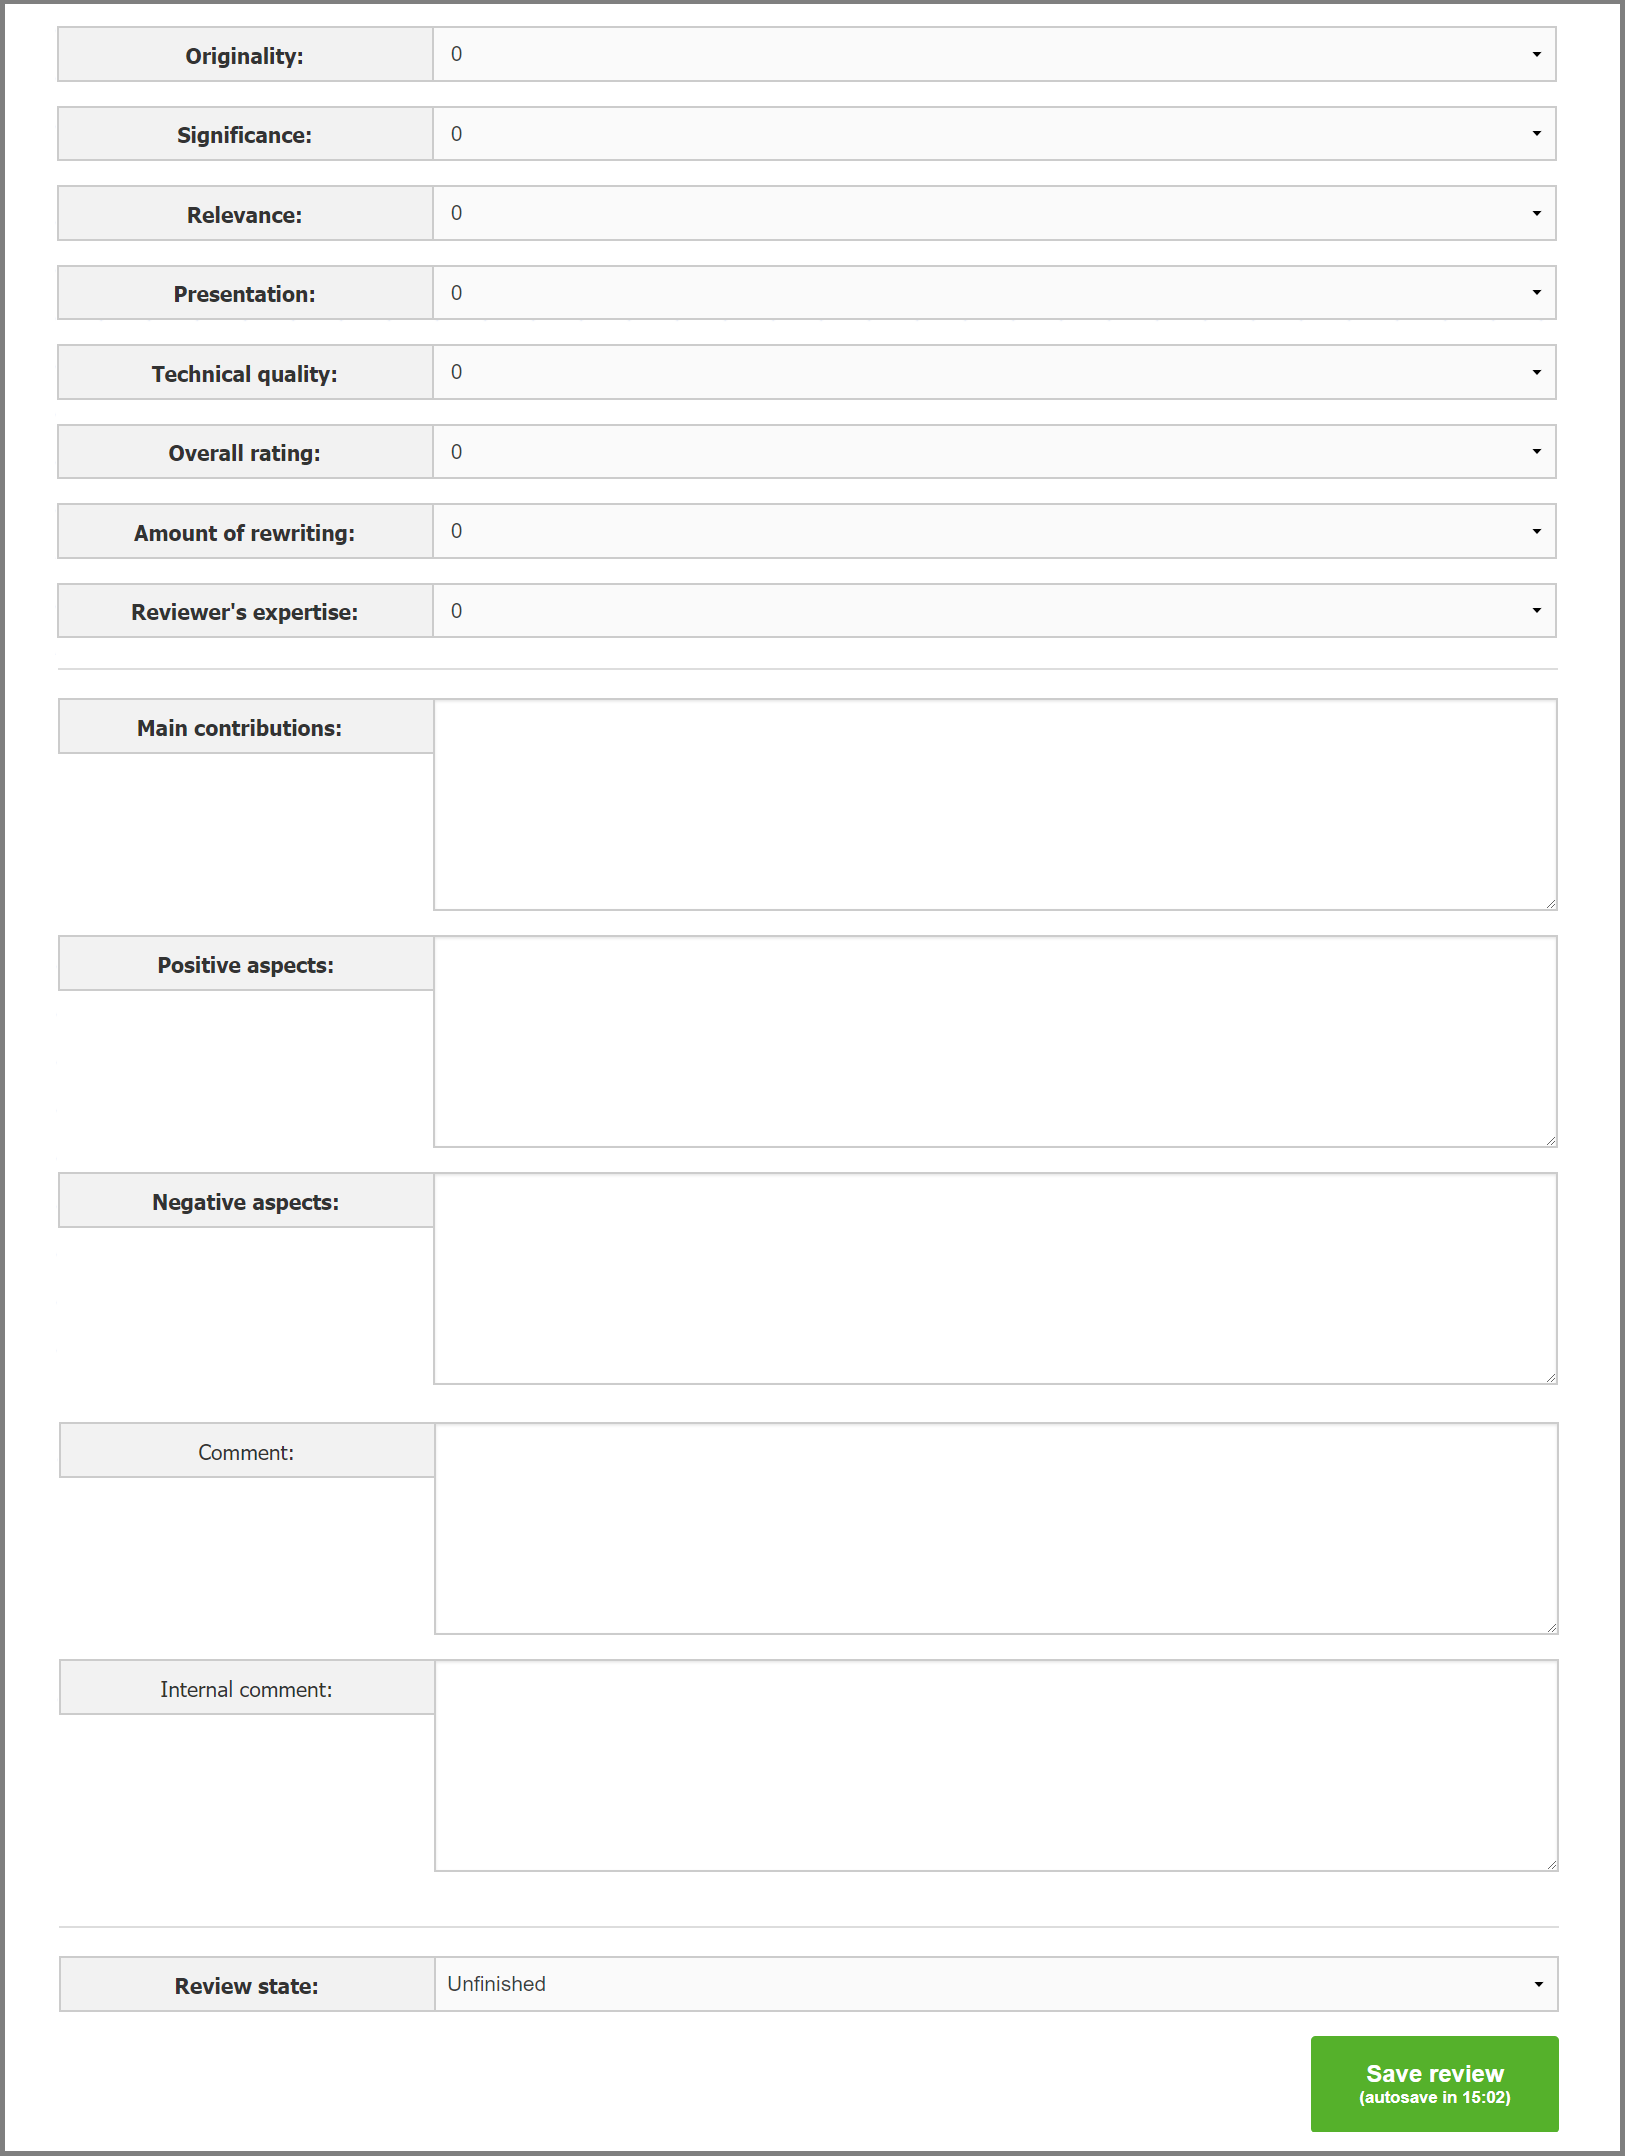
\includegraphics[width=15cm]{img/web_formular}
\caption{Webový formulář používaný pro hodnocení vědeckých příspěvků na portálu konference TSD}
\label{fig:web_formular}
\end{figure}

%SECTION
\section{Hlavní funkce modulu}
Vyvíjený modul musí být napsán stejným stylem jako je celý webový portál konferenčního systému TSD. Jelikož se na tomto portálu vyskytuje modul, který má stejnou funkcionalitu jako modul vyvíjený autorem bakalářské práce, tak je návrh funkcí jednodušší. Modul vyskytující se na portálu implementuje 3 důležité funkce, které zajišťují veškerou funkcionalitu i přes to, že pro zpracovávání PDF souborů je použit externí program \textit{PDFtk}. Po konzultaci s~vedoucím práce bylo rozhodnuto, že se původní názvy funkcí zachovají a budou pouze změněny jejich parametry. Autorův modul bude tedy ve výsledku obsahovat, stejně jako starý modul, 3 důležité funkce doplněny o~pomocné funkce a konstanty. Všechny hlavní funkce jsou popsány níže.  

%SUBSECTION
\subsection{Funkce pro generování}
Pro generování PDF souboru byla navržena 1 funkce. Tato funkce má za úkol nejdříve nastavit veškeré fonty a styly pro vzhled dokumentu, následně využít vhodný generátor PDF souborů, který vytvoří všechny části dokumentu (vypsané v~kapitole \ref{sec:navrh_vzhledu}) a nabídne uživateli možnost stáhnout si výsledný hodnotící PDF soubor. Návrh hlavičky funkce viz \ref{lst:generate_function}.

\lstset{style=phpstyle}
\begin{lstlisting}[caption = {Návrh hlavičky funkce pro generování PDF souboru}, label = {lst:generate_function}, captionpos=b]
function generate_offline_review_form($rid, $reviewer_name, $sid, $submission_name, $submission_filename)
\end{lstlisting}
Popis vstupních parametrů funkce:
\begin{itemize}
	\item\textcolor{blue}{\textbf{\$rid}} -- ID hodnotícího příspěvku
	\item\textcolor{blue}{\textbf{\$reviewer\_name}} -- Celé jméno posuzovatele
	\item\textcolor{blue}{\textbf{\$sid}} -- ID vědeckého příspěvku
	\item\textcolor{blue}{\textbf{\$submission\_name}} -- Celý název vědeckého příspěvku
	\item\textcolor{blue}{\textbf{\$submission\_filename}} -- Celý název PDF souboru vědeckého příspěvku
\end{itemize}

%SUBSECTION
\subsection{Funkce pro zpracování}
Pro zpracování  PDF souboru byly navrženy 2 funkce, kdy první z~nich má za úkol nahrát celý soubor do konferenčního souboru. Po nahrání souboru začne extrakce dat pomocí vhodných parserů a jejich zpracování. Následně se vše uloží do vhodných struktur a všechny extrahované hodnotící parametry se předají do následující funkce. Návrh hlavičky funkce viz \ref{lst:process_function}.

\begin{lstlisting}[caption = {Návrh hlavičky funkce pro extrakci dat}, label = {lst:process_function}, captionpos=b]
function process_offline_review_form($rid, $sid, $revform_filename)
\end{lstlisting}
Popis vstupních parametrů funkce:
\begin{itemize}
	\item\textcolor{blue}{\textbf{\$rid}} -- ID hodnotícího příspěvku
	\item\textcolor{blue}{\textbf{\$sid}} -- ID vědeckého příspěvku
	\item\textcolor{blue}{\textbf{\$revform\_filename}} -- Celý název PDF souboru hodnotícího příspěvku
\end{itemize}

Druhá funkce pro zpracování PDF souboru má za úkol uložit již extrahované hodnotící parametry do databáze konferenčního systému. Návrh hlavičky funkce viz \ref{lst:upload_function}.

\begin{lstlisting}[caption = {Návrh hlavičky funkce pro uložení dat do databáze}, label = {lst:upload_function}, captionpos=b]
function upload_to_DB_offline_review_form($rid, $values)
\end{lstlisting}
Popis vstupních parametrů funkce:
\begin{itemize}
	\item\textcolor{blue}{\textbf{\$rid}} -- ID hodnotícího příspěvku
	\item\textcolor{blue}{\textbf{\$values}} -- Seznam všech hodnotících parametrů 
\end{itemize}
\DeclarePairedDelimiter\ceil{\lceil}{\rceil}
\DeclarePairedDelimiter\floor{\lfloor}{\rfloor}

%CHAPTER
\chapter{Implementace modulu}
Při implementaci modulu bylo třeba vybrat nejvhodnější knihovnu pro generování PDF souboru a tu následně integrovat s~předem vybraným parserem. Pro snadnější integraci byly vytvořeny nové třídy.
\section{Adresářová struktura modulu}
Adresářová struktura modulu na serveru vypadá následovně:
\begin{itemize}
	\item \textbf{config} -- Adresář obsahující konfigurační soubor \textit{configuration.xml}, ve kterém jsou uložena často měněná data (rok konference, upozorňující informace aj.).  
	\item \textbf{img} -- Adresář obsahující obrázky použité v~dokumentu (logo konference TSD).
	\item \textbf{lib} -- Adresář obsahující zdrojové kódy knihoven třetích stran (generátor a parser).
	\item \textbf{src} -- Adresář obsahující zdrojové kódy vytvořené autorem bakalářské práce.
	\item \textbf{orlib.php} -- Hlavní soubor modulu obsahující všechny 3 stěžejní funkce modulu.
\end{itemize}
%SECTION
\section{Implementované třídy}
Pro modul bylo vytvořeno 7 tříd rozdělených do 4 souborů, které zajišťují veškerou pomocnou funkcionalitu (vytváření formulářových prvků, konstanty aj.) při generování PDF souboru. 
%SUBSECTION
\subsection{Výčtové typy}
\textbf{Výčtový typ} (neboli \textbf{Enum}) je datový typ určený pro uložení konstant programu, kdy každé z~těchto konstant je přiřazena jedna instance výčtu. Ve vytvářeném modulu byly použity 4 třídy jako výčtové typy. 
\par
Třída \textbf{Instruction} uchovává konstanty využité při generování titulku a informací během vyplňování formuláře. Tyto konstanty reprezentují celkem 4 části dokumentu (Záhlaví, Titulek dokumentu, Jméno posuzovatele a Instrukční text pro vyplňování formuláře).
\par
Třída \textbf{FormElements} slouží pouze pro rozlišení použitých objektů na základní prvky formuláře. Zde byly použity prvky \textit{Radiobutton} a \textit{Textové pole}.
\par
Ve třídě \textbf{TextareaInfo} jsou uloženy veškeré konstanty pro hodnotící parametry, které jsou reprezentovány jako \textit{Textová pole}, a pomocné funkce. Každý hodnotící parametr je zde určen třemi konstantami (jednoznačný identifikátor, název a jeho popis). Dále se tu vyskytují 2 konstanty využité při vytváření formulářového prvku pomocí HTML kódu. Tyto konstanty jsou využity i při následném zpracování dokumentu pro všechny formulářové prvky reprezentované jako textová pole. Byla zde vytvořena i funkce \textit{getNotNeededConstants} pro získání nepovinných hodnotících parametrů.
\par
Třída \textbf{RadiobuttonInfo} je téměř totožná s~třídou \textbf{TextareaInfo} s~tím rozdílem, že hodnotící parametry jsou reprezentovány jako \textit{Radiobutton}.
%SUBSECTION
\subsection{Elements}
Hlavním důvodem vzniku této třídy byla snaha nevytvářet formulářové prvky přímo v~hlavní funkci \textit{generate\_offline\_review\_form} ale použít nově vytvořené metody. Pomocí implementovaných metod lze vytvářet textová pole, radiobuttony, textové části dokumentu a načítat vědecký příspěvek.
%SUBSECTION
\subsection{TextConversioner}
V~některých případech jsou název vědeckého příspěvku nebo jméno posuzovatele příliš dlouhé, a proto narušuje vzhled výsledného dokumentu. Problém může nastat i při chybě programátora, pokud by byl instrukční text příliš rozsáhlý. Proto byla vytvořena třída \textbf{TextConversioner}, která má za úkol nejdříve zkontrolovat předaný text a porovnat ho se stanovenými konstantami určujícími maximální délku textu. Pokud je rozsah textu delší než stanovená délka, tak se následně vypočte potřebný font pro vykreslení celého textu pomocí vzorce \eqref{eq:font_size}, která se porovnává se stanovenými konstantami určujícími minimální font. 
\begin{equation}
newFontSize = \floor*{\frac{maxTextLength}{textLength} \cdot fontSize} \label{eq:font_size}
\end{equation}

Pokud je vypočtený font je menší než předem stanovený minimální font, je text zkrácen na velikost vypočtenou pomocí vzorce  \eqref{eq:text_length} a doplněn třemi tečkami na jeho konci. 

\begin{equation}
newLength = \floor*{\frac{oldFontSize}{minFontSize} \cdot textLength} \label{eq:text_length}
\end{equation}
%SUBSECTION
\subsection{ConfigurationData}
Třída načítá veškerý obsah konfiguračního souboru, který následně ukládá do svých proměnných. Data uložená v~konfiguračním souboru slouží pro nastavení textu vodoznaku a jako informační text pro uživatele.
%SECTION
\section{Generátor}
Generátor by měl být při vytváření PDF dokumentu rychlý, vykreslit co nejpřesněji prvky webového formuláře do vygenerovaného dokumentu a nebýt implementačně náročný.
%SUBSECTION
\subsection{TCPDF versus mPDF}
Při analyzování dostupných PHP knihoven pro generování PDF souborů byly nalezeny 2 vyhovující knihovny, které mohou potencionálně splňovat potřebnou funkcionalitu, bohužel pouze jedna může být použita do vyvíjeného modulu. Po vytvoření jednoduchého souboru obsahujícího základní formulářové prvky bylo rozhodnuto, že knihovna \textbf{mPDF} bude použita pro generování PDF souborů. Důvody této volby jsou popsány níže.
\par
Za jeden z~důležitých faktorů lze označit skoro kompletní podporu \textit{CSS3} (Cascading Style Sheets 3) u~\textbf{mPDF}, díky čemuž lze dosáhnout perfektního nastavení stylů pro jednotlivé objekty v~dokumentu. Naproti tomu \textbf{TCPDF} nepodporuje značné množství CSS parametrů, například parametr určující šířku vnějšího okraje prvku, a pro dosažení obdobného výsledku je zapotřebí značné množství jiných parametrů definující styl prvku.
\par
Důležitým faktorem při vytváření PDF dokumentu je rychlost generování a paměťová náročnost. V~tabulce \ref{tab:table_generators} lze vidět porovnání knihoven pro 2  PDF soubory, kdy první PDF obsahovalo hlavně CSS styly, zatímco v~dlouhém PDF byla vytvořena tabulka s~více jak tisíci záznamy.
\begin{table}[h!]
\centering
\begin{tabular}{|l|l|l|l|l|} 
\hline
\textbf{Název} & \multicolumn{2}{l|}{\textbf{Komplexní PDF}} & \multicolumn{2}{l|}{\textbf{Dlouhé PDF}}  \\ 
\hline
               & \textbf{Paměť [MB]} & \textbf{Čas [ms]}     & \textbf{Paměť [MB]} & \textbf{Čas [ms]}   \\ 
\hline
TCPDF (v6.2.13)          & 74                  & 35944                 & 2,3                 & 96350               \\ 
\hline
mPDF   (v7.1.6)           & 14                  & 11316                 & 22,5                & 4120                \\
\hline
\end{tabular}
\caption{Tabulka časové náročnosti a využité paměti při generování}
\label{tab:table_generators}
\end{table}
\par
Posledním a zároveň rozhodujícím faktorem je psaní PHP kódu pro vykreslování obsahu, kdy při vytváření kódu u~\textbf{mPDF} se využívá minimum funkcí pro nastavení parametrů PDF souboru jako jsou například metadata, zatímco veškeré zobrazené elementy a text jsou psány v~HTML stylu, se kterým se snadno pracuje. V~mPDF lze snadno měnit parametry jednotlivých elementů, což bude oceněno hlavně u~parseru. U~\textbf{TCPDF} se zobrazovaný obsah vkládá pomocí předem vytvořených funkcí, přičemž tyto funkce mohou obsahovat mnoho parametrů, které si uživatel obtížně zapamatuje a vždy bude potřebovat patřičnou dokumentaci pro správné použití, což bude zabírat mnoho času při vyvíjení nových modulů.
\par
Na závěr porovnání lze říci, že ve většině případů je vhodné využít pro generování PDF souborů knihovnu \textbf{mPDF}. Pokud by bylo nutné vytvořit dokument například ve stylu knihy s~nulovým využitím CSS stylů a potřebou kvalitního vysázení textu, pak je lepší použít knihovnu \textbf{TCPDF}. 

%SUBSECTION
\subsection{Popis vytvoření dokumentu}
Na samotném začátku generování jsou definovány veškeré proměnné vytvořených tříd. U~proměnné, která reprezentuje třídu \textbf{ConfigurationData}, proběhne i načtení dat z~konfiguračního xml souboru. Dále jsou vytvořeny proměnné reprezentující název vybraného dokumentu a informace o~nahrání vyplněného dokumentu do webového portálu konference TSD. Před samotným začátkem generování je do modulu importováno CSS nastavení pro vzhled celého dokumentu.
\par
V~první části generování probíhá vytvoření záhlaví. Pro celý dokument je použit font \textit{Helvetica}, pouze vyjímečně je zařazen font \textit{Times New Roman}, například pro titulek dokumentu a text se stylem \textit{Bold}. Do záhlaví byl vložen identifikátor hodnotícího příspěvku doplněn o~název hodnoceného vědeckého příspěvku, který je případně zkrácen na určitou délku, pokud nesplňuje limity nastavené ve třídě \textbf{TextConversioner}, a logo konference TSD. 
\par
V~druhé části generování proběhlo vložení vodoznaku do celého dokumentu, uložení jednoznačného identifikátoru jak hodnoceného vědeckého příspěvku, tak i hodnotícího příspěvku do příslušných metadat dokumentu. Na první stránce dokumentu je vykreslen titulek s~identifikátorem hodnoceného vědeckého příspěvku, název hodnoceného vědeckého příspěvku (případně zkrácen stejně jako u~záhlaví), jméno posuzovatele a doprovodný text při vyplňování hodnotícího formuláře. Pod tímto textem je vykreslena první část hodnotícího formuláře, která obsahuje 8 skupin radio buttonů a 1 textové pole.
\par
Ve třetí a poslední části probíhá vykreslování zbylých čtyř textových polí, kde 2 poslední z~nich jsou nepovinná. Za hodnotícím formulářem je vložen kompletně celý hodnocený vědecký příspěvek, jehož obsah se uloží do modulu a následně stránku po stránce je přidáván do generovaného PDF dokumentu.
%SUBSECTION
\subsection{Nedostatky v~mPDF}
Při vytváření dokumentu byly nalezeny 2 chyby znemožňující úplné vykreslení celého dokumentu. Níže jsou tyto chyby popsány i s~návrhem jejich řešením.
\par
První nedostatek byl zjištěn na úplném začátku implementace generátoru, kdy při vkládání textových polí do formuláře se po přeložení kódu nevytvořil žádný dokument. Při zkoumání zdrojového kódu knihovny a vytvoření testovacích dokumentů bylo zjištěno, že knihovna neumožňuje použít textové pole, pokud se při jeho vytvoření nezadá vkládaný text. Proto bylo nutné upravit kód knihovny, konkrétně ve vykreslování textového pole. Aby bylo možné takto upravovat zdrojový kód knihovny, tak nesmí být knihovna pod licencí a naopak musí  být alespoň pod licencí dovolující úpravy, například \textit{GNU General Public License} verze 2, pod kterou je licencována i mPDF. Pro vyřešení tohoto problému byl přidán mechanismus, který při vytváření prázdného textového pole přidá znak \uv{\textbf{a}} (viz \ref{lst:elements_a}) a posléze je v~knihovně při vykreslování textového pole tento znak odstraněn, což nemá vliv na jakýkoliv jiný znak či slova než zmiňovaný znak \uv{\textbf{a}}, viz \ref{lst:mpdf_a}.
\begin{lstlisting}[caption = {Dočasné přiřazení znaku \uv{\textbf{a}} do textového pole (Elements.php)}, label = {lst:elements_a}, captionpos=b]
if($textarea_text == '') $textarea_text = 'a';
\end{lstlisting}
\begin{lstlisting}[caption = {Odstranění znaku \uv{\textbf{a}} z~textového pole (Mpdf.php)}, label = {lst:mpdf_a}, captionpos=b]
if (isset($objattr['text']) && $objattr['text'] != 'a') {
	$texto = $objattr['text'];
}
else $texto = '';
\end{lstlisting}
\par
Druhý nedostatek byl nalezen při testování zkracování délky textu titulku, pokud překročí nastavenou mez. V~aktuální verzi PHP se vyskytuje problém, který zneplatňuje některé UTF-8 znaky. Pokud je například vytvořen nový uživatel se jménem obsahující například znak \uv{\textbf{ř}}, pak se tento znak nepřevede správně a bude vykreslen jako neznámý znak. Bohužel generování dokumentu neprobíhalo správně, protože knihovna mPDF tyto znaky nerozpoznala, a proto výsledek vždy skončil chybou. Ze všech vyzkoušených možností, jako například změna kódování textu titulku nebo nahrazení neplatných znaků prázdnými, fungovala pouze jedna, a to nastavení atributu \textbf{ignore\_invalid\_utf8} na \textit{true} u~proměnné třídy \textit{Mpdf} (viz \ref{lst:ignore_invalid_utf8}).
\begin{lstlisting}[caption = {Nastavení atributu \textbf{ignore\_invalid\_utf8} (orlib.php)}, label = {lst:ignore_invalid_utf8}, captionpos=b]
$mpdf->ignore_invalid_utf8 = true;
\end{lstlisting}
\par
Nejzávažnější nedostatek knihovny mPDF byl objeven na samém konci testování. Bylo testováno především slučování hodnotícího formuláře s~vědeckými příspěvky. Vědecké příspěvky byly uloženy ve formátu PDF v~různých verzích, nejčastěji verze 1.4 až 1.6. Testování probíhalo perfektně pro PDF verze 1.4, bohužel pro novější verze už slučování neprobíhalo správně a modul vyhazoval výjimku. Důkladným zkoumáním mPDF knihovny bylo zjištěno, že pro slučování PDF souborů se využívá podpůrná knihovna \textbf{FPDI}, která funguje pouze pro PDF soubory do verze 1.4. V~kapitole \ref{subsec:nova_PDF_merge_knihovna} je popsán postup řešení tohoto nedostatku, který zapříčiňuje nefuknční generování hodnotícího PDF dokumentu.

%SUBSECTION
\subsection{Nová knihovna pro slučování PDF souborů}
\label{subsec:nova_PDF_merge_knihovna}
Jedna z~podmínek pro generující knihovnu je umět vkládat hodnocený vědecký příspěvek do výsledného hodnotícího PDF dokumentu. Protože již implementovaná knihovna FPDI tuto funkci neumožňuje, bude potřeba najít a implementovat jinou knihovnu splňující slučování PDF dokumentů. V~ideálním případě by měla být nově zvolená knihovna kompatibilní s~knihovnou mPDF.
\par
Po rozsáhlém průzkumu byla nalezena pouze jedna PHP knihovna, která dokáže slučovat PDF dokumenty nad verzi 1.4. Je jím knihovna \textbf{TCPDI parser}, která je součástí knihovny \textbf{TCPDI}, která dokáže slučovat PDF do verze 1.7. Jediný požadavek pro správné fungování TCPDI parseru je nutné mít uloženo ve stejné složce filtry z~TCPDF.
\par
Následně byla knihovna FPDI nahrazena TCPDI parserem a otestována na několika testovacích PDF souborech s~rozdílnou PDF verzí. Výsledek sloučení nebyl zrovna přívětivý. Všechny použité styly nebyly přeneseny do výsledného PDF, odsazení textu bylo natolik špatné, že občas byl text posunut mimo stránku.  Bohužel veškeré přílohy, jako jsou například obrázky, komentáře nebo vzorce, nebyly přítomny ve výsledném PDF dokumentu. Na základě těchto problémů bylo rozhodnuto změnit generovací knihovnu. 

%SUBSECTION
\subsection{Změna knihovny pro generování PDF souborů}
Změna knihovny pro generování PDF souborů byla nutná z důvodu nedokonalosti mPDF při slučování více PDF souborů, která nebyla na první pohled vidět. Při testování byla objevena nová knihovna TCPDI, která rozšiřuje již existující knihovnu TCPDF o nové funkce při slučování dvou či více PDF souborů. 
\par
Pro zprovoznění TCPDI je nutné, aby byla na serveru přítomna knihovna TCPDF, do které bude následně vložen zdrojový kód TCPDI. Zdrojový kód TCPDI se skládá ze tří souborů. První soubor \textbf{tcpdi\_parser.php} obsahuje třídu \textit{tcpdi\_parser}, která zpracovává raw kód PDF souboru a ukládá ho do předem stanovených struktur. Druhý soubor \textbf{tcpdi.php} obsahuje třídu \textit{TCPDI}, která rozšiřuje stávající třídu TCPDF a umožňuje slučovat raw kód PDF souborů, ze kterého následně zobrazí výsledný PDF soubor. Třetí a zároveň poslední soubor \textbf{fpdf\_tpl.php} obsahuje třídu \textit{fpdf\_tpl}, která vytváří základy pro znovupoužití PDF objektů v PDF souboru.
\par
Pro generování obsahu PDF souboru se nevytváří HTML kód, ale využívají se předem vytvořené metody. Jako příklad lze uvést metodu \textit{TextField} třídy TCPDI pomocí které se do souboru vloží textové pole. TCPDI obsahuje metodu, která umožnuje generovat PDF soubor i pomocí HTML kódu, ale z důvodu nedostatečné podpory CSS stylů je tento způsob generování nedoporučován. Proto bylo nutné kompletně přepsat již vytvořený zdrojový kód generátoru a co nejvíce se přiblížit vzhledu PDF souboru jako tomu bylo u mPDF. Starý zdrojový kód využívající knihovnu mPDF byl zachován pro případ, že bude vytvořena nová knihovna, která bude schopna slučovat PDF soubory nehledě na verzi PDF a bude kompatibilní s mPDF. 

%SECTION
\section{Parser}
Z~analýzy knihoven pro zpracování PDF dokumentů splnil nutné požadavky pouze \textbf{PDF Parser}.Při implementování parseru bylo zjištěno, že jednotlivé PDF prohlížeče při uložení PDF dokumentu využívají jiné komprimační metody, pracující s~novějšími verzemi PDF pro určité funkce a některé prohlížeče ukládají objekty v~dokumentu na více místech (duplikace, jednou komprimovaně, jednou nekomprimovaně).

%SUBSECTION
\subsection{Popis zpracování dokumentu}
Zpracování dokumentu začíná ihned po jeho nahrání do webového portálu konferenčního systému, kdy se veškerá raw data předají do PDF Parseru. Před samotnou extrakcí dat jsou pomocí TCPDF parseru, který je součástí PDF Parseru, raw data rozdělena na objekty pomocí \textit{traileru} a \textit{xref tabulky}. Následně jsou objekty dekódovány a předány PDF Parseru, který s~nimi dále pracuje. Ihned po předání jsou tyto objekty dále zpracovávány podle specifických znaků, které se vyskytují v~datech, například v~objektu \textit{Slovník} se na samém začátku vyskytují znaky \uv{<<}. Zároveň se kontroluje název objektu, podle kterého lze zjistit o~jaký typ formulářového prvku se jedná. Každý prvek formuláře má přiřazen jednoznačný název. Jako příklad lze uvést textové pole, které má při generování přiřazen název \uv{textareaID}, kde ID je jednoznačný identifikátor textového pole, který je deklarován ve výčtovém typu \textbf{TextareaInfo}. Pokud je název totožný se specifickým názvem jakéhokoliv formulářového prvku, který je v~modulu naimplementován, tak je potom ihned uložen do struktury, která je po dokončení parsování poslána do modulu. 
\par
Po zpracování celého dokumentu jsou požadované objekty roztříděny na základě jejich jednoznačných identifikátorů (čísla na konci slovního identifikátoru, například \uv{\textit{textarea\textbf{0}}}, kde \textbf{0} popisuje v~modulu hodnotící parametr \textit{Originality}). Před uložením hodnot jsou tyto parametry testovány, jestli jsou náležitě vyplněny, což platí pouze pro povinné položky. Zpracování probíhá pro každý základní prvek formuláře samostatně ideálně pomocí cyklu a switche. V~případě, že všechna povinná pole jsou vyplněna a neproběhla žádná chyba ve zpracování, jsou všechny hodnotící parametry uloženy do databáze webového portálu konference TSD.
\par
Při nahrávání dokumentu může dojít k~několika chybám, kterých se posuzovatel může dopustit, a proto jsou náležitě ošetřeny.
\begin{itemize}
	\item \textbf{Neplatné PDF} -- Posuzovatel při nahrávání dokumentu zvolí nevalidní PDF dokument (nevygenerovaný webovým portálem).
	\item \textbf{Neplatný identifikátor hodnotícího příspěvku} -- Posuzovatel může při nahrávání zvolit hodnotící PDF dokument patřící k~jinému hodnocení vědeckého příspěvku (posuzovaní identifikátoru hodnotícího příspěvku a vědeckého příspěvku).
	\item \textbf{Nevyplněné požadované parametry} -- Nahrávaný PDF dokument obsahuje nevyplněné povinné hodnotící parametry. Tyto parametry jsou vypsány v~chybovém hlášení zobrazeném po pokusu nahrát PDF dokument do webového portálu.
	\item \textbf{Databázové chyby} -- Při ukládání dat do databáze webového portálu může dojít k~neočekávané chybě, která zapříčiní nesprávné uložení dat. 
	\item \textbf{Uzavřené hodnocení příspěvku} -- Posuzovatel nahraje hodnotící PDF dokument do webového portálu, zatímco hodnocení vědeckého příspěvku je uzavřeno administrátorem webového portálu.
\end{itemize}

%SUBSECTION
\subsection{Extrakce formulářových prvků z~předpřipravených dat}
TCPDF parser částečně extrahuje veškeré PDF objekty do svých struktur, které jsou následně poslány do PDF Parseru, který je pomocí svých funkcí a tříd rozdělí na základě datového typu vyplněného obsahu, jako je například prostý text, datum nebo číselná hodnota. Příklad struktury jednotlivých objektů lze vidět na obrázku \ref{fig:parsing_object}. Tento obrázek ukazuje pouze část struktury, která je mnohem rozsáhlejší a každým krokem parseru se rozkládá na menší díly.

\begin{figure}[h!]
\centering
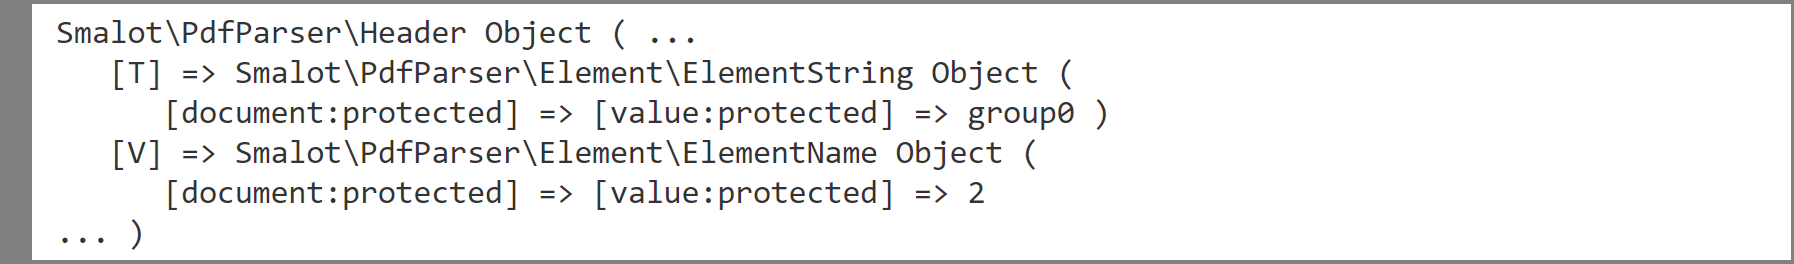
\includegraphics[width=15cm]{img/parsing_object}
\caption{Část dat PDF objektu}
\label{fig:parsing_object}
\end{figure}
\par
Pro extrahování dat a zjištění typu formulářového prvku byla vyvinuta metoda \textit{extractElement} viz \ref{lst:extraction_function}.
\begin{lstlisting}[caption = {Funkční kód pro uložení formulářových prvků z~PDF objektů}, label = {lst:extraction_function}, captionpos=b]
protected function extractElement($header) {
   $elementKey = $header->getElements()['T'];                                                      
   if ($elementKey != null) {
      if (strpos($elementKey->getContent(), 'group') !== false) $type = 'groups';
      else if (strpos($elementKey->getContent(), 'textarea') !== false) $type = 'textareas';
                       
      if ($type != null) {
         $key = $elementKey->getContent();
         $elementValue = $header->getElements()['V'];
         if ($elementValue != null) {
            $value = $elementValue->getContent();
         }    
      }
   }
}
\end{lstlisting}
Kód na samém začátku kontroluje, zda je aktuálně zpracovávaný objekt pojmenován. To je zjištěno na základě indexu \uv{\textbf{T}} (T - Type) v~poli elementů. Pokud název existuje, zjišťuje se zda se jedná o~textové pole nebo skupinu radio buttonů. Za předpokladu, že typ objektu je validní, je kontrolována hodnota na základě indexu \uv{\textbf{V}} (V~- Value) v~poli elementů. Jakmile objekt obsahuje hodnotu, jsou do parseru vráceny všechny tři hodnoty (název formulářového prvku, typ formulářového prvku a jeho hodnota), které parser uloží do pole všech extrahovaných prvků.

%SECTION
\section{Výsledný vzhled PDF formuláře}
Výsledný vzhled PDF formuláře lze vidět na přiloženém PDF souboru v~kapitole \ref{chap:vysledny_vzhled_formulare}. Před formulářem je instrukčí text vysvětlující hodnocení prvních 8 hodnotících parametrů. Protože se v~některých případech stávalo, že uživatelé otevřeli tento dokument ve webovém prohlížeči, který umožňuje pouze otvírat soubory, nikoliv ukládat, byl zde přidán pokyn využívat PDF prohlížeč Adobe Acrobat, ale je možné využívat i jiné prohlížeče, které podporují vyplňování formulářů. Na konec formuláře byl přidán informační text popisující, jak má uživatel vyplněný formulář nahrát do webového portálu konference TSD. Obsah vědeckého příspěvku zde nebyl přidán z~důvodu nevhodnosti prezentování práce někoho jiného.

%SECTION
\section{Technické požadavky}
Technické požadavky pro bezproblémové fungování TCPDI a PDF Parser jsou:
\begin{itemize} 
	\item \textbf{PHP verze} --TCPDI  momentálně funguje na všech verzích PHP, zatímco u~PDF Parseru je potřeba minimální verze 5.3. Proto je nutné mít na serveru PHP verzi alespoň 5.3.0.
	\item \textbf{Podpůrné knihovny} -- Při kompresi stránek PDF souborů pomocí knihovny TCPDI je potřeba mít na serveru povoleno rozšíření \textbf{php-zlib}.
	\item \textbf{FPDF\_TPL verze} -- Aktuální verze TCPDI je kompatibilní pouze s verzí 1.2.3 knihovny FPDF\_TPL. 
\end{itemize}

%CHAPTER
\chapter{Rozšiřitelnost modulu}
Modul je naimplementovaný tak, aby byl snadno rozšiřitelný o nové funkcionality. Zadání bakalářské práce sice splněno bylo, ale v blízké budoucnosti můžou být požadavky na modul změněny. Jako příklad lze uvést potřebu změnit typy hodnotících formulářových prvků (například změna radio buttonů na checkboxy), změnu typu fontu ze základního na speciální, který není přítomen v modulu a mnoho dalšího. V této kapitole jsou popsány 3 možné návrhy na rozšíření modulu, především generátoru.

%SECTION
\section{Podpora ostatních formulářových prvků}
V modulu jsou momentálně podporovány 2 formulářové prvky, a to Textové pole a Radio button. Pro přidání podpory jakéhokoliv formulářového prvku je potřeba splnit několik implementačních kroků. Pro ukázku bude uvedeno vytvoření podpory pro prvek Checkbox.
\par
Jako první je potřeba vytvořit nový výčtový typ s názvem \textbf{CheckboxInfo}. Jednotlivé hodnotící parametry budou obsahovat jednoznačný identifikátor, název a popisek. Dále se vytvoří metoda \textit{getConstants}, která bude mít návratovou hodnotu pole všech hodnotících parametrů. Důležité při vytváření je nadefinovat konstanty reprezentující název prvku při jeho vytváření v HTML kódu. Pro checkboxy bude název například \textit{checkbox} a \textit{checkboxes} (použito při ukládání hodnot u parsování).
\par
Při vytváření HTML kódu reprezentující určitý formulářový prvek se vytvoří nová metoda vracející HTML kód. V tomto kódu bude použit text \textit{checkbox} jako název každého checkboxu (lze použít i pro skupinu, záleží na programátorovi) doplněn o identifikátor určující počet již vytvořených checkboxů. Tento identifikátor je vhodno vytvořit na začátku třídy \textbf{HTMLElements}.
\par
Při parsování je potřeba přidat tento typ do podporovaných prvků v nově implementované metodě \ref{lst:extraction_function}, kde se při kontrole typu přidá nový příkaz \textit{else if}.
\par
Po parsování je potřeba vytvořit nové pole, do kterého se uloží extrahované hodnoty spolu s novým polem, které bude obsahovat data roztříděná na základě jména hodnotícího parametru. Pole extrahovaných se následně roztřídí a nevalidní hodnoty se uloží do společného pole nevalidních prvků (pouze u povinných prvků). Pokud bude zvoleno kritérium povinný prvek/nepovinný prvek, je nutno tyto parametry zkontrolovat nad rámec klasické kontroly. Je to z důvodu toho, že při nevyplnění/nezvolení hodnoty hodnotícího parametru nebude tento parametr reprezentován v poli všech prvků daného typu formulářového prvku a při ukládání hodnoty do databáze nebude stávající hodnota přepsána. Pokud bude jeden z povinných prvků nevalidních, je potřeba zjistit které a přidat ho do chybového hlášení pro uživatele.
\par
Pokud jsou všechny povinné hodnoty extrahovány a uloženy, jsou následně uloženy do databáze. Proto je potřeba správně hodnoty z daného prvku přiřadit ke správné hodnotě.

%SECTION
\section{Změna fontu}
V celém dokumentu jsou využity 2 typy fontů - hlavní font \textit{Helvetica} je použit pro veškerý netučný text, zatímco font \textit{Times New Roman} je využit pro veškeré tučné písmo.
\par
Pokud je potřeba změnit font netučného písma, tak je nutné změnit parametr \textit{default\_font} reprezentující typ fontu při vytváření proměnné třídy \textbf{Mpdf} v metodě \textit{setMPDF}. V případě, že chce programátor použít speciální typy fontů vytvořené třetí stranou, pak je potřeba stáhnout \textit{TrueType} (koncovka .ttf) soubor s definovanými styly a vložit ho do složky \textit{ttfonts}, která se nachází v mPDF složce. Pro využívání tučného písma, kurzívu a tučnou kurzívu daného typu fontu, je potřeba stáhnout ke každému stylu extra soubor. Následně je potřeba vytvořit záznam ve třídě \textit{FontVariables} taktéž v knihovně mPDF viz \ref{lst:font_define}.
\begin{lstlisting}[caption = {Nový záznam fontu v knihovně mPDF}, label = {lst:font_define}, captionpos=b]
'fontdata' => [
   "timesnewroman" => [
      'R' => "TimesNewRoman.ttf",
      'B' => "TimesNewRomanBold.ttf",
      'I' => "TimesNewRomanItalic.ttf",
      'BI' => "TimesNewRomanBoldItalic.ttf",
      'useOTL' => 0xFF,
   ],
],
\end{lstlisting}
\par
Pro změnu tučného písma v PDF dokumentu je nutné změnit atribut určující typ fontu v CSS souboru \textit{style.css}. Tučné písmo je použito především na názvy hodnotících parametrů a titulek dokumentu.

%SECTION
\section{Načtení nově přidaných dat z konfiguračního souboru}
Konfigurační soubor \textit{configuration.xml} obsahuje data, která se můžou častěji měnit v průběhu hodnocení bez nutnosti přepisovat zdrojový kód modulu. Pro přidání nového záznamu je nutné dodržovat stanovený postup:
\begin{enumerate}
	\item Vytvoření nového elementu a přiřadit mu text.
	\item Vytvoření nové proměnné ve třídě \textit{ConfigurationData}.
	\item Načtení dat pomocí XML readeru implementovaného v PHP. Při získávání dat elementu je nutné dodržovat styl \textit{\$reader->nazev\_elementu}. 
\end{enumerate}
%CHAPTER
\chapter{Ověření kvality software}
Po vytvoření modulu je nutné ověřit kvalitu řešení. Testování bylo zaměřeno hlavně na kvalitu vygenerovaného dokumentu PDF a jeho následné zpracování. Pro tento účel byl vytvořen testovací scénář pro recenzenta vědeckých příspěvků. Důležitým faktorem při testování vytvořeného modulu je otestovat kompatibilitu s~nejvíce využívanými webovými a prohlížeči PDF. Vyplněné testovací scénáře se nachází v~příloze bakalářské práce.

%SECTION
\section{Testování modulu}

%SUBSECTION
\subsection{Generování souboru PDF}
Pro generování a stažení dokumentu bylo použito šest nejčastěji využívaných webových prohlížečů.
\par
Jako první testované prohlížeče lze zmínit \textit{Microsoft Edge (v42.17134.1.0)} a \textit{Internet Explorer (v11)} firmy Microsoft, které jsou již předinstalované na všech operačních systémech Windows od verze 10. Stažení proběhlo zcela v~pořádku, při stahování je potřeba zvolit možnost stažení souboru do počítače, nikoliv pouze otevření souboru. Vygenerovaný soubor PDF obsahoval všechny potřebné části pro hodnocení vědeckého příspěvku. Formulář bylo možné editovat.
\par
Generování bylo testováno i na webových prohlížečích \textit{Mozilla Firefox (v66.0.2)} a \textit{Google Chrome (v73.0.3683.103)}. Testování probíhalo na dvou operačních systémech Windows 10 a Linux (Ubuntu v18.04.1 LTS, Kernel 4.15.0--44--generic. I~zde proběhlo generování a stažení dokumentu bez sebemenších problémů, kdy Google Chrome ihned po stažení otevřel výchozí prohlížeč souborů PDF, zatímco Mozilla Firefox nabídl možnost stažení či pouze otevření souboru PDF. Stejně jako tomu bylo u~prvních dvou webových prohlížečů, bylo nutno soubor stáhnout, nikoliv pouze otevřít. Vygenerovaný soubor obsahoval editovatelný formulář i vědecký příspěvek, který je posuzován.
\par
Poslední dva webové prohlížece, na kterých bylo generování souboru PDF testováno, jsou \textit{Safari (v5.1.7)} a \textit{Opera (v58)}. Testování probíhalo pouze na systému Windows. Po stažení byl soubor PDF ihned otevřen výchozím prohlížečem PDF. Formulář byl editovatelný, veškeré části hodnotícího souboru PDF zde byly přítomny.
\par
Protože chytré telefony má dnes skoro každý, bylo proto nutné otestovat generování souboru PDF i na operačních systémech \textit{Android (v4.2.1 -- Jelly Bean)} a \textit{iOS (v12.2)}. Bez sebemenších problémů byl hodnotící soubor PDF vygenerován. Hodnotící formulář byl editovatelný.

%SUBSECTION
\subsection{Vyplnění a zpracování souboru PDF}
Při vyplnění vygenerovaného hodnotícího souboru PDF bylo použito sedm prohlížečů PDF, viz \ref{tab:table_zpracovani}. K~nahrání vyplněného souboru PDF byl použit webový prohlížeč Google Chrome.

\begin{table}[h!]
\centering
\begin{tabular}{|l|l|l|l|} 
\hline
\textbf{Prohlížeč PDF} & \textbf{Verze PDF} & \textbf{Interaktivní formulář} & \textbf{Uložení hodnot}  \\ 
\hline
Adobe Acrobat Reader   & 1.6.0                & Ano                            & Ano                      \\ 
\hline
Adobe Acrobat Pro      & 1.6.0                & Ano                            & Ano                      \\ 
\hline
Evince                 & 1.4.0                & Ano                            & Ano                      \\ 
\hline
PDFElements            & 1.4.0                & Ano                            & Ano                      \\ 
\hline
Nitro Pro              & 1.4.0                & Ano                            & Ano                      \\ 
\hline
Sumatra                & X                  & Ne                             & Ne                       \\ 
\hline
Foxit - Linux          & 1.4.0                & Ano                            & Ano                      \\ 
\hline
Evince - Linux         & 1.4.0                & Ano                            & Ano                      \\
\hline
\end{tabular}
\caption{Prohlížeče PDF použité při testování}
\label{tab:table_zpracovani}
\end{table}

\par
Nejčastěji využívané prohlížeče PDF jsou \textit{Adobe Acrobat Reader} a \textit{Adobe Acrobat Pro} ve verzi v19.01.020091. Hodnotící formulář zde byl editovatelný, obrázky se vyskytují v~perfektní kvalitě a při ukládání byla použita verze PDF 1.6.0. Po nahrání souboru PDF v~recenzním řízení do webového portálu konference TSD byly všechny vyplněné hodnoty extrahovány a úspěšně uloženy do databáze.
\par
Mezi známější prohlížeče PDF lze zařadit i \textit{Evince (v3.32)}, který byl použit pro testování na operačních systémech \textit{Windows 10} a \textit{Linux}. Vzhled formulářových prvků zde vypadal trochu jinak než jak tomu bylo u~Adobe prohlížečů, při ukládání souboru PDF byla použita verze PDF 1.4.0. Nahrání souboru a extrahování potřebných hodnot proběhlo bez sebemenších problémů na obou operačních systémech.
\par
Mezi méně známé prohlížeče PDF lze zařadit \textit{PDFElements (v6)}, \textit{Nitro Pro (v12)} a \textit{Foxit (v9.4.1.16828)}. Všechny tyto prohlížeče bezproblémově uložily všechny vyplněné hodnoty ve verzi PDF 1.4.0. Stejně jako tomu bylo u~\textit{Evince}, i zde se nevyskytl žádný problém při nahrávání souboru a extrakci požadovaných hodnot.
\par
Jako poslední prohlížeč PDF byl použit prohlížeč \textit{Sumatra (v3.1.2)}. Sumatra nepodporuje editovatelné formuláře, slouží pouze k~prohlížení souborů PDF. Proto z~tohoto důvodu nelze použít prohlížeč Sumatra pro vygenerovaný soubor PDF v~recenzním řízení.

%SUBSECTION
\subsection{Nalezené chyby při testování}
\label{subsec:chyby_pri_testovani}
Při testování modulu se objevily dvě větší chyby, které nebyly zapříčiněné použitou knihovnou. Jednalo se o~chyby při zpracovávání nahraného souboru PDF.
\par
První chyba byla objevena při testování knihovny TCPDI. Při kontrole extrahovaných hodnot z~nahraného souboru PDF se u~každé skupiny přepínacích tlačítek kontroluje, zda obsahuje hodnotu \uv{Off}. Pokud obsahuje, pak uživatel nezvolil ani jednu možnost v~dané skupině přepínacích tlačítek. Bohužel tento postup fungoval pouze u~formulářů vygenerovaných knihovnou mPDF, nikoliv u~formulářů vygenerovaných knihovnou TCPDI. U~TCPDI se při nezvolené možnosti ve skupině přepínacích tlačítek se daný hodnotící prvek ani neextrahuje, tudíž není dostupný a nelze ho nijak zkontrolovat. Proto byla přidána kontrola, zda extrahovaná data obsahují všechny hodnotící parametry u~všech formulářových prvků.
\par
Druhá chyba byla nalezena při ukládání hodnot do databáze. V~hodnotícím formuláři se vyskytují parametry, které uživatel nemusí vyplňovat. Pokud tyto položky nejsou vyplněné, nejsou při nahrávání extrahovány a následně uloženy do databáze, tudíž při nahrání nového souboru PDF se stávalo, že zde zůstali z~předchozího hodnocení komentáře. Proto bylo nutné zjistit zda tyto nepovinné parametry jsou vyplněny a pokud ne, byly explicitně vytvořeny v~modulu s~přiřazenou hodnotou, která byla prázdný řetězec. Tímto způsobem byly přepsány všechny parametry z~minulého hodnocení.

%SECTION
\section{Testovací scénář}
Testovací scénář je orientován především na vzhled celého dokumentu a rozložení jeho jednotlivých částí. Dále byly položeny otázky na bezproblémové ovládání modulu (vygenerování a nahrání dokumentu PDF). Poslední otázka byla zaměřena na poznámky a připomínky ohledně vytvořeného modulu, které by do budoucna mohly posloužit při případném rozšiřování modulu.
Výsledný testovací scénář předložený uživatelům konferenčního systému TSD obsahuje tyto otázky:
\begin{itemize}
	\item \textbf{Vyskytly se nějaké problémy při stahování či nahrávání dokumentu PDF?}
	\item \textbf{Jak byste ohodnotil vzhled dokumentu jako celek?}
	\item \textbf{Jak hodnotíte vzhled formuláře a použité prvky reprezentující jednotlivé hodnotící parametry?}
	\item \textbf{Byla velikost textového pole dostatečně velká pro případné komentáře ohledně vědeckého příspěvku?}
	\item \textbf{Jak hodnotíte rychlost stažení a nahrání dokumentu PDF?} 
	\item \textbf{Byly Vámi vyplněné hodnoty správně nahrány do webového portálu?}
	\item \textbf{Děkuji za vyplnění dotazníku. Pokud máte jakékoliv další poznámky, připomínky či návrhy, uveďte je, prosím, zde:}
\end{itemize}

%SECTION
\section{Výsledky uživatelského testování}
Funkčnost modulu byla otestována dvěma uživateli webového portálu konference TSD. Níže jsou popsány souhrny jednotlivých částí testovacího reportu. V~kapitole \ref{chap:testovaci_reporty} jsou podrobně rozepsány všechny odpovědi uživatelu.
%SUBSECTION
\subsection{Vzhled dokumentu PDF}
Vzhled hodnotícího formuláře byl podle uživatelů vcelku přehledný a věcný, ale svým vzhledem je ani neurazil, ani nenadchnul. Velikost textových polí byla dostatečně velká pro zadání všech informací. Ohledně celkového vzhledu dokumentu měli uživatelé námitku na odsazení výběrových tlačítek. Ocenili by především větší odsazení skupin výběrových tlačítek od ostatních sekcí.
%SUBSECTION
\subsection{Nalezené chyby a připomínky}
Při stahování a nahrávání dokumentů se nevyskytly žádné problémy a vše proběhlo bez výraznějších prodlev mezi jedna až dvěmi vteřinami. Při nahrávání vyplněného souboru PDF v~recenzním řízení do webového portálu se u~prvního uživatele vyskytly problémy, zatímco druhý neměl žádné připomínky. Připomínky prvního uživatele byly: portál nezná háčky, čárky a opravuje je na nesmyslné znaky, je schopný nahrát i nesmyslný text ve stylu samých teček a problém při ukládání hodnot do databáze, který spočíval v~přepisování starých hodnot novými. Co se týče špatného zobrazování háčků a čárek tak tento problém byl vysvětlen v~kapitole \ref{subsec:nedostatky_v_mpdf}. Ohledně nesmyslného textu, většina hodnotících parametrů je povinná, a proto musí být i v~off-line formuláři náležitě vyplněny všechny povinné parametry. Poslední připomínka byla zjištěna ke konci autorova testování, kdy už byly rozeslány testovací reporty všem uživatelům, viz kapitola \ref{subsec:chyby_pri_testovani}.  

  
%CHAPTER
\chapter{Závěr}
 

%%%%%%%%%%%%%%%%%%%%%%%%%%%%%%%%%%%%%%%%%%%%%%%%%%%%%%%%%%
%
% LITERATURA
%
%%%%%%%%%%%%%%%%%%%%%%%%%%%%%%%%%%%%%%%%%%%%%%%%%%%%%%%%%%
\bibliographystyle{csplainnatkiv}
{\raggedright\small
\bibliography{literature/literatura}
}

%%%%%%%%%%%%%%%%%%%%%%%%%%%%%%%%%%%%%%%%%%%%%%%%%%%%%%%%%%
%
% PŘÍLOHA
%
%%%%%%%%%%%%%%%%%%%%%%%%%%%%%%%%%%%%%%%%%%%%%%%%%%%%%%%%%%
\setcounter{chapter}{0}
\renewcommand{\thechapter}{\Alph{chapter}}

%CHAPTER
\chapter{Uživatelská dokumentace}
Pro nasazení modulu na webový server je potřeba provést tyto kroky:
\begin{enumerate}
	\item V~kořenovém adresáři serveru nebo v~aktuálním pracovním adresáři je potřeba vytvořit složky \textbf{php} a \textbf{php/offline-review}.
	\item Přesunout celý modul do adresáře \textbf{php/offline-review}.
	\item V~souboru \textit{orlib.php} přepsat konstantu \uv{DATA\_ROOT} na aktuální pracovní adresář či kořenový adresář (přednastavený pracovní adresář je definován v~konfiguračním souboru webového portálu konference TSD).
\end{enumerate}


Postup pro uživatele při využití tohoto modulu:
\begin{enumerate}
	\item Přihlášení do webového portálu konference TSD.
	\item Přesunout se do záložky \uv{My Reviews}.
	\item Vybrat si ze seznamu jeden vědecký příspěvek a kliknout na příslušné tlačítko pro otevření hodnotícího formuláře (\uv{Review} tlačítko).
	\item Pod textem \uv{Offline review form} (v~pravé horní části webového prohlížeče) lze vidět 2 tlačítka:
	\begin{itemize}
		\item Levé tlačítko (obrázek bez zelené šipky) má za úkol vygenerovat příslušný hodnotící soubor k~aktuálně hodnocenému vědeckému příspěvku.
		\item Pravé tlačítko (obrázek se zelenou šipkou) má za úkol zpracovat příslušný hodnotící soubor a nahrát do databáze extrahované hodnotící parametry.
	\end{itemize}
\end{enumerate}
 
%CHAPTER
\chapter{Testovací reporty}
\label{chap:testovaci_reporty}

%SECTION
\section{Tester 1}

\textbf{Vyskytly se nějaké problémy při stahování či nahrávání PDF dokumentu?}
\newline
První
\newline
\newline
\textbf{Jak by jste ohodnotil vzhled dokumentu jako celek?}
\newline
Druhá
\newline
\newline
\textbf{Jak hodnotíte vzhled formuláře a použité prvky reprezentující jednotlivé hodnotící parametry?}
\newline
Třetí
\newline
\newline
\textbf{Byla velikost textového pole dostatečně velká pro případně komentáře ohledně vědeckého příspěvku?}
\newline
Čtvrtá
\newline
\newline
\textbf{Jak hodnotíte rychlost stažení a nahrání PDF dokumentu?} 
\newline
Pátá
\newline
\newline
\textbf{Byly Vámi vyplněné hodnoty správně nahrány do webového portálu?}
\newline
Šestá
\newline
\newline
\textbf{Děkuji za vyplnění dotazníku. Pokud máte jakékoliv další poznámky, připomínky či návrhy, uveďte je prosím zde:}
\newline
Sedmá
\newpage 

%SECTION
\section{Tester 2}

\textbf{Vyskytly se nějaké problémy při stahování či nahrávání PDF dokumentu?}
\newline
První
\newline
\newline
\textbf{Jak by jste ohodnotil vzhled dokumentu jako celek?}
\newline
Druhá
\newline
\newline
\textbf{Jak hodnotíte vzhled formuláře a použité prvky reprezentující jednotlivé hodnotící parametry?}
\newline
Třetí
\newline
\newline
\textbf{Byla velikost textového pole dostatečně velká pro případně komentáře ohledně vědeckého příspěvku?}
\newline
Čtvrtá
\newline
\newline
\textbf{Jak hodnotíte rychlost stažení a nahrání PDF dokumentu?} 
\newline
Pátá
\newline
\newline
\textbf{Byly Vámi vyplněné hodnoty správně nahrány do webového portálu?}
\newline
Šestá
\newline
\newline
\textbf{Děkuji za vyplnění dotazníku. Pokud máte jakékoliv další poznámky, připomínky či návrhy, uveďte je prosím zde:}
\newline
Sedmá
\newpage 

%CHAPTER
\chapter{Vzhled PDF formuláře}
\label{chap:vysledny_vzhled}
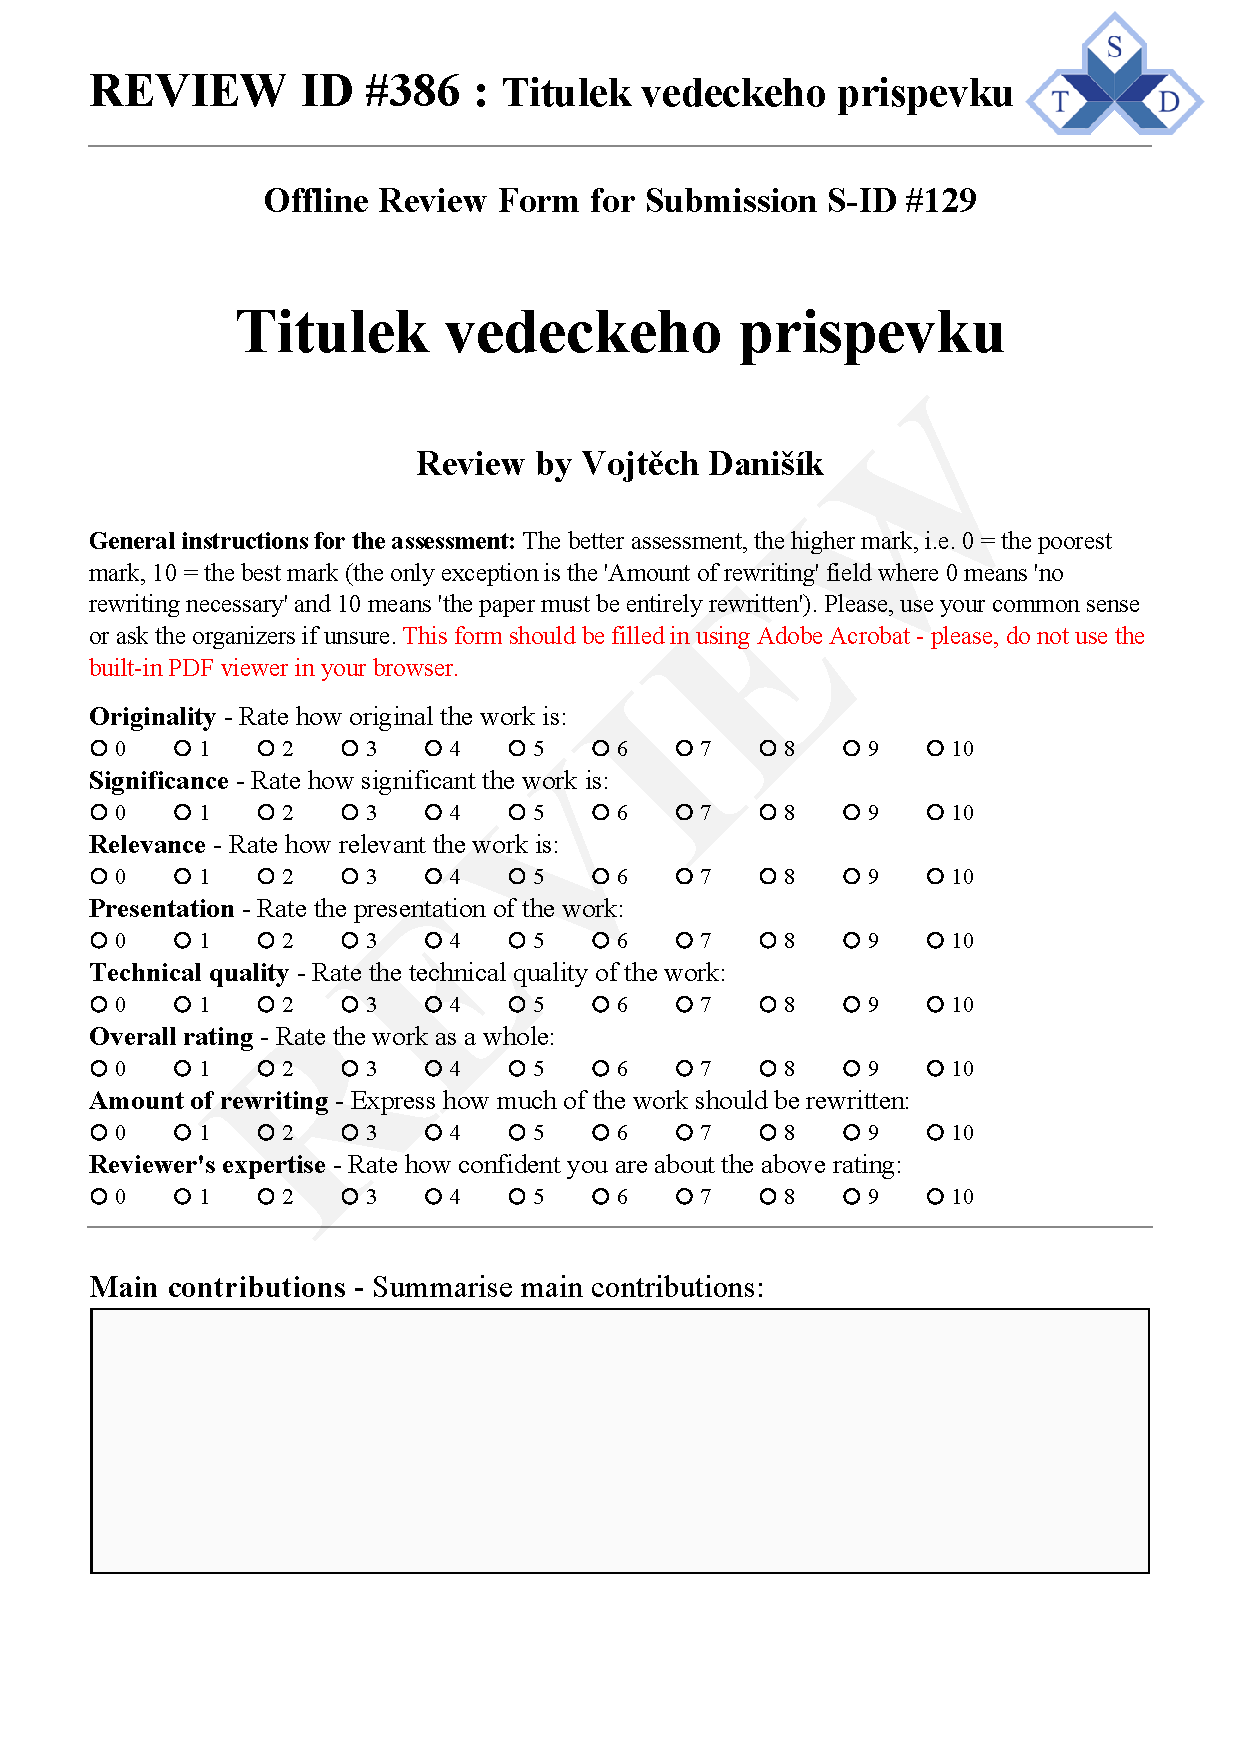
\includepdf[pages=1,pagecommand={},width=1.3\textwidth]{pdf/vysledny_vzhled.pdf}
\includepdf[pages=2,pagecommand={},width=1.3\textwidth]{pdf/vysledny_vzhled.pdf}

%%%%%%%%%%%%%%%%%%%%%%%%%%%%%%%%%%%%%%%%%%%%%%%%%%%%%%%%%%
%
% KONEC TEXTU PRÁCE
%
%%%%%%%%%%%%%%%%%%%%%%%%%%%%%%%%%%%%%%%%%%%%%%%%%%%%%%%%%%
\end{document}
